\subsection{多项式代数上的复合算子}

设 K 为特征 0 的交换域，K{[}X{]} 为 K 上一个未定元的多项式代数（Alg., IV. 1）；在本节中，我们把 K{[}X{]} 上的算子理解为向量空间 K{[}X{]} （在 K 上）到其自身的线性映射 U；由于单项式 \(X^{n}\) （ \(n \geqslant 0\) ）构成此空间的一组基，U 由多项式 \(U(X^{n})\) 确定；确切地说，若 \(f(X) = \sum_{k=0}^{\infty} \lambda_{k} X^{k}\) ，其中 \(\lambda_{k} \in K\) ，则 \(U(f) = \sum_{k=0}^{\infty} \lambda_{k} U(X^{k})\) 。

若 \(\mathbf{G}\) 是 \(\mathbf{K}\) 上的一个含单位元的交换代数，则 \(\mathbf{G}\) -模 \(\mathrm{G}[\mathrm{X}]\) 是由把 \(\mathbf{K}\) -向量空间 \(\mathrm{K}[\mathrm{X}]\) 的标量域扩张到 \(\mathrm{G}\) 而得到的；每个算子 \(U\) （定义在 \(\mathrm{K}[\mathrm{X}]\) 上）都以唯一的方式扩张为 \(\mathrm{G}\) -模 \(\mathrm{G}[\mathrm{X}]\) 到其自身的一个线性映射，我们仍将它记作 \(U\) （Alg., II, p.~278）；对每个元素 \(g(\mathrm{X}) = \sum_{k=0}^{\infty} \gamma_k X^k\) ，其中 \(\gamma_k \in \mathrm{G}\) ，有 \(U(g) = \sum_{k=0}^{\infty} \gamma_k U(X^k)\) 。

特别地，考虑 \(\mathrm{G} = \mathrm{K}[\mathrm{Y}]\) 的情形；这时 \(\mathrm{G}[\mathrm{X}]\) 是环 \(\mathrm{K}[\mathrm{X},\mathrm{Y}]\) ，即 \(\mathrm{K}\) 上两个未定元的多项式环；为避免混淆，我们把 \(U\) 到 \(\mathrm{G}[\mathrm{X}]\) 上的扩张记作 \(U_{\mathrm{X}}\) 。于是，对任意多项式 \(g(\mathrm{X},\mathrm{Y}) = \sum_{k=0}^{\infty}\gamma_k(\mathrm{Y})\mathrm{X}^k\) （其中 \(\gamma_k(Y)\in \mathrm{K}[\mathrm{Y}]\) ）有 \(U_{\mathrm{X}}(g) = \sum_{k=0}^{\infty}\gamma_k(\mathrm{Y})U(\mathrm{X}^k)\) 。由于 \(U_{\mathrm{X}}\) 是线性的，可以看出，若把它写成 \(g(\mathrm{X},\mathrm{Y}) = \sum_{h=0}^{\infty}\beta_h(\mathrm{X})\mathrm{Y}^h\) ，则也有 \(U_{\mathrm{X}}(g) = \sum_{h=0}^{\infty}U(\beta_h)\mathrm{Y}^h\) 。

在把 X 对应到 Y 的 K{[}X{]} 到 K{[}Y{]} 上的典范同构下，算子 U 变换为 K{[}Y{]} 上的一个算子；为避免混淆，我们把它记作 \(U_{Y}\) ，于是 \(U_{\mathrm{Y}}(f(\mathrm{Y}))\) 就是在多项式 \(U(f(\mathrm{X})) = U_{\mathrm{X}}(f(\mathrm{X}))\) 中把 X 换成 Y 所得到的多项式。这个算子 \(U_{Y}\) 又可以扩张为一个算子（仍记作 \(U_{Y}\) ），它定义在 K{[}X,Y{]} 上：若 \(g(\mathrm{X}, \mathrm{Y}) = \sum_{h=0}^{\infty} \beta_{h}(\mathrm{X}) \mathrm{Y}^{h}\) ，则 \(U_{\mathrm{Y}}(g(\mathrm{X}, \mathrm{Y})) = \sum_{h=0}^{\infty} \beta_{h}(\mathrm{X}) U_{\mathrm{Y}}(\mathrm{Y}^{h})\) 。

作为这些扩张的一个例子，我们举出 K{[}X{]} 上的求导算子 D （Alg., IV. 6），它给出偏求导算子 \(D_{X}\) 与 \(D_{Y}\) （定义在 K{[}X,Y{]} 上）。

对每个多项式 \(f \in K[X]\) ，我们用 \(T_{Y}(f)\) 表示多项式 \(f(X + Y)\) （它属于 K{[}X,Y{]}）；映射 \(T_{Y}\) 是从 K{[}X{]} 到 K{[}X,Y{]} 中的一个 K-线性映射，称为平移算子。

定义 1. 称 K{[}X{]} 上的算子 U 为复合算子，如果它与平移算子可交换，也就是说，如果 \(U_{X}T_{Y} = T_{Y}U\) 。

换句话说，若 \(f\) 是 \(\mathbf{K}[\mathbf{X}]\) 中的任意一个多项式，且 \(g = U(f)\) ，则必须有 \(g(\mathbf{X} + \mathbf{Y}) = U_{\mathbf{X}}(f(\mathbf{X} + \mathbf{Y}))\) 。

由这个定义立即得出，对每个多项式 \(f(\mathrm{X}) \in \mathrm{K}[\mathrm{X}]\) ，按上述记号有

\[
U _ {\mathrm{X}} \big (f (\mathrm{X} + \mathrm{Y}) \big) = U _ {\mathrm{Y}} \big (f (\mathrm{X} + \mathrm{Y}) \big).\tag{1}
\]

例. 1) 对每个 \(\lambda \in \mathbf{K}\) ，把每个多项式 \(f(\mathbf{X})\) 对应到多项式 \(f(\mathbf{X} + \lambda)\) 的算子是一个复合算子。

\begin{enumerate}
\def\labelenumi{\arabic{enumi})}
\setcounter{enumi}{1}
\tightlist
\item
  K{[}X{]} 上的求导 D 是一个复合算子（参见命题 1）。
\end{enumerate}

注. 由于 K 是无限域，K{[}X{]} 上的算子 U 是复合算子，当且仅当对每个多项式 \(f \in K[X]\) 和每个元素 \(\alpha \in K\) ，令 \(g = U(f)\) ，有 \(g(X + \alpha) = U(f(X + \alpha))\) 。（Alg., IV. 16, cor.）

显然，复合算子的以 K 为系数的每个线性组合仍是复合算子；两个复合算子的复合（乘积）也是如此。换句话说，复合算子构成一个子代数 \(\Gamma\) ，含于向量空间 K{[}X{]} 的自同态代数中。

命题 1. K{[}X{]} 上的算子 U 是复合算子的充分必要条件为：它与 K{[}X{]} 上的求导 D 可交换。

事实上，泰勒公式表明，对每个多项式 \(f \in K[X]\) 有

\[
U _ {\mathrm{X}} \big (f (\mathrm{X} + \mathrm{Y}) \big) = U _ {\mathrm{X}} \left(\sum_ {k = 0} ^ {\infty} \frac {1}{k !} \mathrm{Y} ^ {k} \mathrm{D} ^ {k} f (\mathrm{X})\right) = \sum_ {k = 0} ^ {\infty} \frac {1}{k !} \mathrm{Y} ^ {k} U \big (\mathrm{D} ^ {k} f (\mathrm{X}) \big);
\]

若令 \(g = U(f)\) ，则有

\[
g (\mathrm{X} + \mathrm{Y}) = \sum_ {k = 0} ^ {\infty} \frac {1}{k !} \mathrm{Y} ^ {k} \mathrm{D} ^ {k} g (\mathrm{X}) = \sum_ {k = 0} ^ {\infty} \frac {1}{k !} \mathrm{Y} ^ {k} \mathrm{D} ^ {k} (U (f (\mathrm{X})))
\]

于是，为使 U 是复合算子，必须有 \(UD^{k} = D^{k}U\) （对每个整数 \(k \geqslant 1\) ），特别地有 \(UD = DU\) 。反之，若这一关系成立，则由对 k 的归纳法，它蕴含 \(UD^{k} = D^{k}U\) （对每个整数 \(k \geqslant 1\) ）；于是泰勒公式表明 \(g(X + Y) = U_{X}(f(X + Y))\) 。

对每个多项式 \(f \in K[X, Y]\) ，我们用 \(U_{0}(f)\) 表示多项式 \(U_{X}(f)\) 中不含 X 的项；特别地，若 \(f \in K[X]\) ，则 \(U_{0}(f)\) 是 \(U(f)\) 中的常数项，而 \(U_{0}\) 是 K{[}X{]} 上的一个线性型。对每个多项式 \(f \in K[X]\) ，令 \(g = U(f)\) ；由 VI, p.~270 的定义 1

\[
g (\mathrm{X} + \mathrm{Y}) = U _ {\mathrm{X}} (f (\mathrm{X} + \mathrm{Y})) = U _ {\mathrm{X}} \left(\sum_ {k = 0} ^ {\infty} \frac {1}{k !} \mathrm{X} ^ {k} \mathrm{D} ^ {k} f (\mathrm{Y})\right) = \sum_ {k = 0} ^ {\infty} \frac {1}{k !} U (\mathrm{X} ^ {k}) \mathrm{D} ^ {k} f (\mathrm{Y})
\]

而若在这个公式中把 X 换成 0 ，就得到

\[
g (\mathrm{Y}) = \sum_ {k = 0} ^ {\infty} \frac {1}{k !} U _ {0} (\mathrm{X} ^ {k}) \mathrm{D} ^ {k} f (\mathrm{Y}).
\]

于是可以看出

\[
U (f (\mathrm{X})) = \sum_ {k = 0} ^ {\infty} \frac {1}{k !} \mu_ {k} \mathrm{D} ^ {k} f (\mathrm{X})\tag{2}
\]

其中 \(\mu_{k}\) 是多项式 \(U(\mathbf{X}^k)\) 的常数项。

这个公式表明，诸 \(\mu_{k}\) 完全确定了复合算子 U；反过来，若 \((\mu_{n})\) 是 K 中元素的一个任意序列，则公式 (2) 定义了一个算子 U，它显然与 D 可交换，因而（VI, p.~270, prop. 1）是一个复合算子。今后我们把 (2) 写成如下形式

\[
U = \sum_ {k = 0} ^ {\infty} \frac {1}{k !} \mu_ {k} D ^ {k}.\tag{3}
\]

这个公式可以用拓扑语言解释如下：若在 K{[}X{]} 上考虑离散拓扑，并在自同态代数 \(\operatorname{End}(\operatorname{K}[X])\) （由 K{[}X{]} 的自同态组成）上考虑单收敛拓扑（Gen.~Top., X, p.~277），则以 \(\frac{1}{k!}\mu_{k}D^{k}\) 为通项的级数在 \(\operatorname{End}(\operatorname{K}[X])\) 中交换收敛，且其和为 U （Gen.~Top., III, p.~269）。

公式 (3) 表明，对形式级数 \(u(S) = \sum_{k=0}^{\infty} \alpha_k S^k\) （\(K\) 上一个未定元的，Alg., IV. 41），可以对应一个复合算子 \(U = \sum_{k=0}^{\infty} \alpha_k D^k\) ，今后我们把它记作 \(u(D)\) 。这一注记可以按如下方式加以阐明：

定理 1. 把每个形式级数 \(u(\mathbf{S}) = \sum_{k=0}^{\infty} \alpha_k \mathbf{S}^k\) （\(\mathbf{K}\) 上一个未定元的）对应到复合算子 \(u(\mathbf{D}) = \sum_{k=0}^{\infty} \alpha_k \mathbf{D}^k\) （\(\mathrm{K}[\mathrm{X}]\) 上的）的映射，是形式级数代数 \(\mathrm{K}[[\mathrm{S}]]\) 到复合算子代数 \(\Gamma\) 上的一个同构。

立即可以验证这个映射是一个同态。剩下要证的是它是单射，换句话说，关系 \(\sum_{k=0}^{\infty}\alpha_{k}D^{k}=0\) 蕴含对每个 k 都有 \(\alpha_{k}=0\) ；而 \(h!\alpha_{h}\) 是把 \(\sum_{k=0}^{\infty}\alpha_{k}D^{k}\) 作用于 \(X^{h}\) 所得多项式的常数项，由此即得定理。

推论. 复合算子代数 \(\Gamma\) （K{[}X{]} 中的）是交换的。

例. 若 \(U\) 是把每个多项式 \(f(\mathrm{X})\) 对应到 \(f(\mathrm{X} + \lambda)\) （其中 \(\lambda \in \mathbf{K}\) ）的算子，则有 \(U_0(\mathrm{X}^k) = \lambda^k\) ，从而 \(U = \sum_{k=0}^{\infty} \frac{1}{k!} (\lambda \mathrm{D})^k\) 。与 \(e^x\) 的级数展开（III, p.~105）相类比，我们用 \(e^{\mathrm{S}}\) 或 \(\exp(\mathrm{S})\) 表示形式级数 \(\sum_{n=0}^{\infty} \frac{1}{n!} \mathrm{S}^n\) （环 \(\mathrm{K}[[\mathrm{S}]]\) 中的）；于是可以写 \(U = e^{\lambda \mathrm{D}}\) 。在这论证中把域 \(\mathrm{K}\) 换成有理分式域 \(\mathrm{K}(\mathrm{Y})\) ，同样可以看出平移算子 \(T_{\mathrm{Y}}\) 可写成 \(e^{\mathrm{YD}}\) 。

此外，在 K 上两个未定元的形式级数环 K{[}{[}S, T{]}{]} 中有

\[
\begin{array}{l} (\exp S) (\exp T) = \sum_ {p, q} \frac {S ^ {p}}{p !} \frac {T ^ {q}}{q !} \\ = \sum_ {n = 0} ^ {\infty} \frac {1}{n !} \left(\binom {n} {0} S ^ {n} + \binom {n} {1} S ^ {n - 1} T + \dots + \binom {n} {n} T ^ {n}\right) \\ = \exp (S + T) \end{array}\tag{4}
\]

特别地，有

\[
(\exp S) (\exp (- S)) = 1\tag{5}
\]

这就说明我们引入的记号是合理的。

按语. 形式级数代数 K{[}{[}S{]}{]} 与复合算子代数 \(\Gamma\) （K{[}X{]} 上的）之间的同构，有时使我们能用对相应的复合算子证明命题的办法，最简单地证明关于形式级数的命题（参见 VI, p.~274, prop. 6）。

\subsection{与复合算子相联系的阿佩尔多项式}

给定一个复合算子 \(U = \sum_{k=0}^{\infty} \alpha_k \mathrm{D}^k \neq 0\) ，设 \(p\) 为整数 \(k\) （使 \(\alpha_k \neq 0\) 的）中最小的一个；我们称 \(p\) 为算子 \(U\) 的阶。

命题 2. 每个 0 阶复合算子在复合算子代数 \(\Gamma\) （K{[}X{]} 上的）中可逆。

事实上，形式级数 \(\sum_{k=0}^{\infty}\alpha_{k}S^{k}\) （满足 \(\alpha_{0}\neq0\) ）在环 K{[}{[}S{]}{]} 中可逆（Alg., IV. 41）；于是命题由 VI, p.~271 的定理 1 得出。

命题 3. 设 U 是一个 p 阶复合算子；则 \(U(f) = 0\) （对每个次数 \textless{} p 的多项式 f）；对每个多项式 \(f \neq 0\) （次数 \(n \geqslant p\) 的），\(U(f)\) 是一个次数为 n - p 的多项式 \(\neq 0\) 。

这是 VI, p.~271 的公式 (2) 与 \(U\) 的阶的定义的直接推论。

显然，每个算子 \(U\) （\(p\) 阶的）都可以以唯一的方式写成 \(U = \mathrm{D}^p V = V\mathrm{D}^p\) ，其中 \(V\) 是一个 0 阶算子（从而可逆）。

定义 2. 设 \(U = \mathrm{D}^p V\) 是一个 \(p\) 阶复合算子（\(\mathrm{K}[\mathrm{X}]\) 上的）。多项式 \(u_n(\mathrm{X}) = V^{-1}(\mathrm{X}^n)\) 称为指标为 \(n\) 而与算子 \(U\) 相联系的阿佩尔多项式。

\[
\text {   If   } V ^ {- 1} = \sum_ {k = 0} ^ {\infty} \frac {1}{k !} \beta_ {k} D ^ {k} (\text {   with   } \beta_ {0} \neq 0) \text {   one   thus   has   }
\]

\[
u _ {n} (\mathrm{X}) = \sum_ {k = 0} ^ {n} {\binom {n} {k}} \beta_ {k}   \mathrm{X} ^ {n - k}.\tag{6}
\]

可以验证 \(u_{n}\) 是一个 \(n\) 次多项式（prop. 3）；此外

\[
u _ {n} (0) = \beta_ {n}.
\]

命题 4. 与 \(U\) 相联系的阿佩尔多项式满足下列关系

\[
\frac {d u _ {n}}{d \mathrm{X}} = n u _ {n - 1}\tag{7}
\]

\[
u _ {n} (\mathrm{X} + \mathrm{Y}) = \sum_ {k = 0} ^ {n} {\binom {n} {k}} u _ {n - k} (\mathrm{X})   \mathrm{Y} ^ {k}\tag{8}
\]

\[
U \left(u _ {n} (\mathrm{X})\right) = \frac {n !}{(n - p) !} \mathrm{X} ^ {n - p}.\tag{9}
\]

这些公式事实上分别等价于下列关系（记住定义 2）：

\[
\mathbf {D} V ^ {- 1} = V ^ {- 1} \mathbf {D}\tag{10}
\]

\[
\left(\exp \left(\mathrm{YD} _ {\mathrm{X}}\right)\right) V _ {\mathrm{X}} ^ {- 1} = V _ {\mathrm{X}} ^ {- 1} \exp \left(\mathrm{YD} _ {\mathrm{X}}\right)\tag{11}
\]

\[
U V ^ {- 1} = \mathbf {D} ^ {p}.\tag{12}
\]

命题 5. 对每个多项式 \(f \in \mathrm{K}[\mathrm{X}]\) 和每个复合算子 \(U\) （\(p\) 阶的），有

\[
f ^ {(p)} (\mathrm{X} + \mathrm{Y}) = \sum_ {k = 0} ^ {\infty} \frac {1}{k !} U (f ^ {(k)} (\mathrm{X})) u _ {k} (\mathrm{Y})\tag{13}
\]

（广义泰勒展开）。

事实上，若令 \(U = \mathrm{D}^p V = V\mathrm{D}^p\) ，则有（VI, p.~270, 公式 (1)）

\[
V _ {\mathrm{X}} ^ {- 1} (f (\mathrm{X} + \mathrm{Y})) = V _ {\mathrm{Y}} ^ {- 1} (f (\mathrm{X} + \mathrm{Y})) = \sum_ {k = 0} ^ {\infty} \frac {1}{k !} f ^ {(k)} (\mathrm{X}) u _ {k} (\mathrm{Y})\tag{14}
\]

这是由泰勒公式及 VI, p.~273 的定义 2 得到的；只需对公式 (14) 的首末两项应用算子 \(U_{\mathrm{X}}\) 即得 (13)。

\subsection{阿佩尔多项式的生成级数}

设 E 为一个未定元 S 的形式级数环，其系数取在多项式环 K{[}X{]} 中（Alg., IV. 41）；换句话说，即形式级数 \(g(\mathrm{X}, \mathrm{S}) = \sum_{n=0}^{\infty} \alpha_n(\mathrm{X}) \mathrm{S}^n\) 组成的环，其中诸 \(\alpha_n\) 属于 K{[}X{]}。对每个算子 \(U\) （K{[}X{]} 上的），定义 E 到其自身的一个映射 \(U_{\mathrm{X}}\) 如下：置 \(U_{\mathrm{X}}(g(\mathrm{X}, \mathrm{S})) = \sum_{n=0}^{\infty} U(\alpha_n)\mathrm{S}^n\) 。显然，E 是以 K 为系数的未定元 S 的形式级数环 K{[}{[}S{]}{]} 上的一个模；由 \(U\) 在 K{[}X{]} 上的线性性，立即可以验证，对每个元素 \(\theta \in \mathrm{K}[[\mathrm{S}]]\) 和每个 \(g \in \mathrm{E}\) ，有 \(U_{\mathrm{X}}(\theta g) = \theta U_{\mathrm{X}}(g)\) ；换句话说，\(U_{\mathrm{X}}\) 是模 E 到其自身中的一个线性映射。

命题 6. 设 \(U = D^{p}V = u(D)\) 是 K{[}X{]} 上一个 p 阶复合算子，其中 \(u(S)\) 是 K{[}{[}S{]}{]} 中一个 p 阶形式幂级数。则

\[
U _ {\mathrm{X}} \big (\exp (\mathrm{XS}) \big) = u (\mathrm{S}) \exp (\mathrm{XS})\tag{15}
\]

\[
\frac {\mathrm{S} ^ {p}}{u (\mathrm{S})} \exp (\mathrm{XS}) = \sum_ {n = 0} ^ {\infty} \frac {1}{n !} u _ {n} (\mathrm{X}) \mathrm{S} ^ {n}\tag{16}
\]

其中 \(u_{n}\) 是与 U 相联系的指标为 n 的阿佩尔多项式。

由定理 1 的按语（VI, p.~271），为建立 (15)，只需证明对每个多项式 \(f(\mathrm{Y}) \in \mathrm{K}[\mathrm{Y}]\) 有

\[
U _ {\mathrm{X}} \left(\exp (\mathrm{XD} _ {\mathrm{Y}}) (f (\mathrm{Y}))\right) = u (\mathrm{D} _ {\mathrm{Y}}) \left(\exp (\mathrm{XD} _ {\mathrm{Y}}) (f (\mathrm{Y}))\right).\tag{17}
\]

而 (17) 中的第一项是 \(U_{\mathrm{X}}(f(\mathrm{X} + \mathrm{Y}))\) ，并且由于 \(U = u(\mathrm{D})\) ，(17) 中的第二项是 \(U_{\mathrm{Y}}(f(\mathrm{X} + \mathrm{Y}))\) ，于是恒等式 (17) 就归结为 (1) （VI, p.~270）。

现在只需把 (15) 应用于复合算子 \(V^{-1} = D^{p}/u(D)\) 即得 (16)，因为按定义有

\[
V ^ {- 1} \big (\exp (\mathrm{XS}) \big) = \sum_ {n = 0} ^ {\infty} \frac {1}{n !} u _ {n} (\mathrm{X}) \mathrm{S} ^ {n}.
\]

注意，把形式级数 \(S^{p}/u(S)\) 与 \(\exp(XS)\) 相乘并利用 (6)，也可以得到 (16)。

我们称形式级数 (16) 为与 U 相联系的阿佩尔多项式的生成级数。

\subsection{伯努利多项式}

考虑由下式定义的复合算子 U

\[
U (f (\mathrm{X})) = f (\mathrm{X} + 1) - f (\mathrm{X});
\]

可以写 \(U = e^{\mathrm{D}} - 1\) （VI, p.~270, 例 1）；这是一个 1 阶算子，且若令 \(U = DV\) ，则有 \(V^{-1} = \frac{\mathrm{D}}{e^{\mathrm{D}} - 1}\) 。\(n\) 次阿佩尔多项式（与算子 \(U\) 相应的）称为 \(n\) 次伯努利多项式，记作 \(\mathrm{B}_n(\mathrm{X})\) ；若令 \(b_n = \mathrm{B}_n(0)\) ，则有公式

\[
\mathrm{B} _ {n} (\mathrm{X}) = \sum_ {k = 0} ^ {n} \binom{n}{k} b _ {n - k} \mathrm{X} ^ {k}\tag{18}
\]

\[
\frac {\mathrm{Se} ^ {\mathrm{XS}}}{e ^ {\mathrm{S}} - 1} = \sum_ {n = 0} ^ {\infty} \frac {1}{n !} \mathrm{B} _ {n} (\mathrm{X}) \mathrm{S} ^ {n}\tag{19}
\]

特别地，有

\[
{\frac {\mathrm{S}}{e ^ {\mathrm{S}} - 1}} = \sum_ {n = 0} ^ {\infty} {\frac {1}{n !}} b _ {n} \mathrm{S} ^ {n}\tag{20}
\]

VI, p.~273 的公式 (7) 和 (9) 给出，对伯努利多项式，有关系

\[
\frac {d \mathrm{B} _ {n}}{d \mathrm{X}} = n \mathrm{B} _ {n - 1} (X)\tag{21}
\]

\[
\mathrm{B} _ {n} (\mathrm{X} + 1) - \mathrm{B} _ {n} (\mathrm{X}) = n \mathrm{X} ^ {n - 1}.\tag{22}
\]

特别地，有 \(\mathrm{B}_{n}(1)-\mathrm{B}_{n}(0)=0\) （对 n\textgreater1），由此并利用 (18)，就得到递推关系

\[
\sum_ {m = 0} ^ {n - 1} \binom {n} {m} b _ {m} = 0 \qquad (\text { for } n > 1)\tag{23}
\]

它使我们能逐步算出诸 \(b_{n}\) 。这些数显然都是有理数；由于可以写

\[
{\frac {S}{e ^ {S} - 1}} = - {\frac {S}{2}} + {\frac {S}{2}} {\frac {e ^ {S} + 1}{e ^ {S} - 1}}
\]

以及由于（VI, p.~272, 公式 (5)）

\[
\frac {e ^ {- S} + 1}{e ^ {- S} - 1} = - \frac {e ^ {S} + 1}{e ^ {S} - 1}
\]

可以看出，在 \(\frac{S}{2}\frac{e^{S}+1}{e^{S}-1}\) 的形式级数中，一切奇数次项的系数均为零；于是有

\[
b _ {0} = 1, \qquad b _ {1} = - \frac {1}{2}, \qquad b _ {2 n - 1} = 0 \quad \text { for } n > 1.\tag{24}
\]

有理数 \(b_{2n}\) （ \(n \geqslant 1\) ）称为伯努利数；我们将看到（VI, p.~288），\(b_{2n}\) 的符号是 \((-1)^{n-1}\) 的符号。公式 (23) 给出，对 n 的前几个值，

\[
\begin{array}{c} b _ {2} = \frac {1}{6}, \quad b _ {4} = - \frac {1}{3 0}, \quad b _ {6} = \frac {1}{4 2}, \quad b _ {8} = - \frac {1}{3 0}, \\ b _ {1 0} = \frac {5}{6 6}, \quad b _ {1 2} = - \frac {6 9 1}{2 7 3 0}, \quad b _ {1 4} = \frac {7}{6}, \\ b _ {1 6} = - \frac {3 6 1 7}{5 1 0}, \quad b _ {1 8} = \frac {4 3 8 6 7}{7 9 8}, \quad b _ {2 0} = - \frac {1 7 4 6 1 1}{3 3 0}, \quad b _ {2 2} = \frac {8 5 4 5 1 3}{1 3 8}, \\ b _ {2 4} = - \frac {2 3 6 3 6 4 0 9 1}{2 7 3 0}, \quad b _ {2 6} = \frac {8 5 5 3 1 0 3}{6}, \quad b _ {2 8} = - \frac {2 3 7 4 9 4 6 1 0 2 9}{8 7 0}. \end{array}
\]

注意 691、3617、43867 这几个分子是素数；其余的素因子分解为

\[
\begin{array}{c} 1 7 4 6 1 1 = 2 8 3 \times 6 1 7 \\ 8 5 4 5 1 3 = 1 1 \times 1 3 1 \times 5 9 3 \\ 2 3 6 3 6 4 0 9 1 = 1 0 3 \times 2 2 9 4 7 9 7 \\ 8 5 5 3 1 0 3 = 1 3 \times 6 5 7 9 3 1 \\ 2 3 7 4 9 4 6 1 0 2 9 = 7 \times 9 3 4 9 \times 3 6 2 9 0 3. \end{array}
\]

由此可导出前几个伯努利多项式的表达式

\[
\mathrm{B} _ {0} (\mathrm{X}) = 1, \quad \mathrm{B} _ {1} (\mathrm{X}) = \mathrm{X} - \frac {1}{2}, \quad \mathrm{B} _ {2} (\mathrm{X}) = \mathrm{X} ^ {2} - \mathrm{X} + \frac {1}{6},
\]

\[
\mathrm{B} _ {3} (\mathrm{X}) = \mathrm{X} ^ {3} - \frac {3}{2} \mathrm{X} ^ {2} + \frac {1}{2} \mathrm{X}, \quad \mathrm{B} _ {4} (\mathrm{X}) = \mathrm{X} ^ {4} - 2 \mathrm{X} ^ {3} + \mathrm{X} ^ {2} - \frac {1}{3 0}.
\]

\subsection{实变函数上的复合算子}

设 I 是 R 中包含区间 \(R_{+} = [0, +\infty[\) 的一个区间；设 E 是复数域 C 上的一个向量空间，由定义在 I 上的复值实变函数组成。我们假设对每个 \(a \geqslant 0\) 和每个函数 \(f \in E\) ，函数 \(x \mapsto f(x + a)\) 属于 E；此外，我们假定 E 包含复系数多项式在 I 上的限制以及指数函数 \(e^{\lambda x}\) ，其中 \(\lambda\) 是任意复数。E 到从 I 到复数域 C 的全体映射所成空间中的任何线性映射 U 都称为 E 上的算子；若 \(f \in E\) 且 \(g = U(f)\) ，使用记号

\[
g (x) = U _ {x} ^ {\xi} \left(f (\xi)\right)
\]

其中 \(\xi\) 是右端函数记号中的哑变量（参见 II, p.~58）。对每个 \(a \geqslant 0\) ，把任意函数 \(f \in E\) 对应到函数 \(x \mapsto f(x + a)\) 在 I 上的限制的算子，称为平移 a 的平移算子。

定义 3. 称 E 上的算子 U 为复合算子，如果对每个 \(a \geqslant 0\) ，它与平移 a 的平移算子可交换。

按上面引入的记号，这个定义成为恒等式

\[
U _ {x + a} ^ {\xi} (f (\xi)) = U _ {x} ^ {\xi} (f (\xi + a))\tag{25}
\]

它是关于 \(x\) 和 \(a\) 的恒等式（ \(x \in \mathrm{I}, a \geqslant 0\) ）。可以在该恒等式中交换 \(x\) 与 \(a\) 的角色，只要 \(x \geqslant 0\) ；然后令 \(a = 0\) ；于是对 \(x \geqslant 0\) 得到

\[
U _ {x} ^ {\xi} (f (\xi)) = U _ {0} ^ {\xi} (f (\xi + x))\tag{26}
\]

其中 \(U_{0}\) 是 E 上的线性型，它把每个函数 \(f \in E\) 对应到值 \(g(0)\) ，其中 \(g = U(f)\) 。

若 \(f\) 是多项式，则有 \(f(\xi + x) = \sum_{k=0}^{\infty} \frac{1}{k!} f^{(k)}(\xi)x^k\) ，且公式 (26) 表明 \(U(f)\) 也是多项式；把它限制在 \(x\) 的多项式所成的集合上（系数在 \(\mathbf{C}\) 中，该集合可与代数 \(\mathbf{C}[\mathbf{X}]\) 等同），算子 \(U\) 就是 VI, p.~270 定义 1 意义下的复合算子，从而前面各节的所有结果都可以应用于它。

我们仍把与算子 U 相联系的阿佩尔多项式记作 \(u_{n}\) 。对更一般的函数，与多项式的广义泰勒展开（VI, p.~274, 公式 (13)）相对应，有下列结果：

定理 2. 设 f 是在 I 上具有连续的 \((n+1)^{th}\) 阶导数、并且与其所有导数 \(f^{(m)}\) （ \(1 \leqslant m \leqslant n\) ）一起都属于 E 的函数。若 U 是 E 上一个 \(p \leqslant n\) 阶的复合算子，则对 \(x \geqslant 0\) 和 \(h \geqslant 0\) 有

\[
f ^ {(p)} (x + h) = \sum_ {m = 0} ^ {n} \frac {1}{m !} u _ {m} (x) U _ {h} ^ {\xi} \left(f ^ {(m)} (\xi)\right) + \mathrm{R} _ {n} (x, h)\tag{27}
\]

其中

\[
\mathrm{R} _ {n} (x, h) = - U _ {h} ^ {\xi} \left(\int_ {0} ^ {\xi - x - h} \frac {1}{n !} u _ {n} (x + \eta) f ^ {(n + 1)} (\xi - \eta) d \eta\right)\tag{28}
\]

（广义泰勒展开）。

考虑积分 \(\int_{0}^{\xi-x-h}\frac{1}{n!}u_{n}(x+\eta)f^{(n+1)}(\xi-\eta)d\eta\) （它对所有 \(\xi\in I\) 有定义），并对它应用 \(n+1\) 阶分部积分公式（II, p.~59, 公式 (11)）；利用关系式

\[
u _ {n} ^ {(k)} = n (n - 1) \dots (n - k + 1) u _ {n - k}
\]

（它们是由 (7) （VI, p.~273）通过递推得到的），就得到

\[
\begin{array}{l} \int_ {0} ^ {\xi - x - h} \frac {1}{n !} u _ {n} (x + \eta) f ^ {(n + 1)} (\xi - \eta) d \eta \\ = \sum_ {m = 0} ^ {n} \frac {1}{m !} u _ {m} (x) f ^ {(m)} (\xi) - \sum_ {m = 0} ^ {n} \frac {1}{m !} u _ {m} (\xi - h) f ^ {(m)} (x + h). \end{array}\tag{29}
\]

我们把算子 U 作用于 (29) 的两边（把它们看作 \(\xi\) 的函数），然后取所得函数在变量 \(\xi\) 之值为 h 处的值；注意到，由公式 (26) （VI, p.~277）和 (9) （VI, p.~272），有

\[
U _ {h} ^ {\xi} \big (u _ {m} (\xi - h) \big) = U _ {0} ^ {\xi} \big (u _ {m} (\xi) \big) = \left\{ \begin{array}{l l} 0 & \text {for} m \neq p \\ p! & \text {for} m = p \end{array} \right.
\]

最终就得到 (27)。

\subsection{复合算子的指示函数}

在与 \(n^{\circ}\) 5 相同的假设下，把（VI, p.~277）的公式 (26) 应用于函数 \(e^{\lambda x}\) ，就得到

\[
U _ {x} ^ {\xi} (e ^ {\lambda \xi}) = U _ {0} ^ {\xi} (e ^ {\lambda x} e ^ {\lambda \xi}) = e ^ {\lambda x} U _ {0} ^ {\xi} (e ^ {\lambda \xi}) = u (\lambda) e ^ {\lambda x}\tag{30}
\]

其中令 \(u(\lambda) = U_{0}^{\xi}(e^{\lambda\xi})\) 。定义在 C 上、取复数值的函数 \(u(\lambda)\) 称为复合算子 U 的指示函数。注意，若 U 在多项式环 C{[}X{]} 上的限制等于级数

\[
\mathbf {D} ^ {p} \sum_ {n = 0} ^ {\infty} \alpha_ {n} \mathbf {D} ^ {n}
\]

\pandocbounded{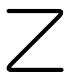
\includegraphics[keepaspectratio]{images/part002_816cd56c.jpg}}

（VI, p.~271, th. 1）（我们在 VI, p.~271 已把它记作 \(u(\mathrm{D})\) ），则以 \(\alpha_{n}\lambda^{n+p}\) 为通项的复数项级数对 \(\lambda \neq 0\) 不一定收敛，而且即使它对 \(\lambda\) 的某些值收敛，其和也不一定等于 U 的指示函数 \(u(\lambda)\) （VI, p.~291, exerc. 2）。若存在 C 中 0 的一个邻域，使得以 \(\alpha_{n}\lambda^{n+p}\) 为通项的级数在其上绝对收敛且其和等于指示函数 \(u(\lambda)\) ，则我们称复合算子 U 为正则的 \(^{1}\) 。把 VI, p.~278 的公式 (27) 应用于函数 \(e^{\lambda x}\) ，取 h = 0；由于 \(\mathrm{D}^{m}(e^{\lambda x}) = \lambda^{m} e^{\lambda x}\) ，有 \(U_{0}^{\xi}\left(\mathrm{D}^{m}(e^{\lambda x})\right) = \lambda^{m} u(\lambda)\) ；由此得出，对每个复数 \(\lambda\) （满足 \(u(\lambda) \neq 0\) 的）

\[
\frac {\lambda^ {p} e ^ {\lambda x}}{u (\lambda)} = \sum_ {m = 0} ^ {n} u _ {m} (x) \frac {\lambda^ {m}}{m !} - \frac {\lambda^ {n + 1}}{u (\lambda)} U _ {0} ^ {\xi} \left(\int_ {0} ^ {\xi - x} \frac {1}{n !} u _ {n} (x + \eta) e ^ {\lambda (\xi - \eta)} d \eta\right)\tag{31}
\]

特别地，对 \(x = 0\) ，有

\[
\frac {\lambda^ {p}}{u (\lambda)} = \sum_ {m = 0} ^ {n} \beta_ {m} \frac {\lambda^ {m}}{m !} - \frac {\lambda^ {n + 1}}{u (\lambda)} U _ {0} ^ {\xi} \left(\int_ {0} ^ {\xi} \frac {1}{n !} u _ {n} (\eta) e ^ {\lambda (\xi - \eta)} d \eta\right)\tag{32}
\]

其中 \(\beta_{m} = u_{m}(0)\) 。

若 \(U\) 是正则算子，则对一切 \(\lambda \in \mathbf{C}\) （使幂级数 \(u(\lambda) = \sum_{n=0}^{\infty} \alpha_n \lambda^{n+p}\) 与 \(\sum_{n=0}^{\infty} \beta_n \frac{\lambda^n}{n!}\) 绝对收敛者）\(^2\) ，由公式 (16) 及两个绝对收敛级数的乘积公式（Gen.~Top., VIII, p.~115, prop. 1），有

\[
{\frac {\lambda^ {p}}{u (\lambda)}} = \sum_ {n = 0} ^ {\infty} \beta_ {n} {\frac {\lambda^ {n}}{n !}}.\tag{33}
\]

同样，由于 \(e^{\lambda x}\) 的泰勒展开对每个 \(\lambda \in \mathbf{C}\) 和每个 \(x \in \mathbf{C}\) 都绝对收敛（III, p.~106），（由公式 (6) （VI, p.~273）与 (16) （VI, p.~274））对所考虑的一切值和一切 \(x \in \mathbf{C}\) 也有

\[
\frac {\lambda^ {p} e ^ {\lambda x}}{u (\lambda)} = \sum_ {n = 0} ^ {\infty} u _ {n} (x) \frac {\lambda^ {n}}{n !}.\tag{34}
\]

注. 可以利用公式 (33) （相应地 (34)），借助下面关于幂级数的引理来计算诸 \(\beta_{n}\) （相应地诸 \(u_{n}(x)\) ）：

引理. 若两个幂级数 \(\sum_{n=0}^{\infty} c_n \lambda^n\) 、\(\sum_{n=0}^{\infty} d_n \lambda^n\) 在 0 的某个邻域内的一切 \(\lambda\) 处绝对收敛，且若 \(\sum_{n=0}^{\infty} c_n \lambda^n = \sum_{n=0}^{\infty} d_n \lambda^n\) 对这些 \(\lambda\) 的值成立，则 \(c_n = d_n\) （对一切整数 \(n \geqslant 0^3\) ）。

若用任何方法能找到一个在 0 的某个邻域上收敛于 \(\lambda^p / u(\lambda)\) 的幂级数，则该级数的系数必然等于诸 \(\beta_n / n!\) 。在下面各例中我们就要应用这个方法。

例. 1) 若 \(U\) 是恒等映射，则有 \(u(\lambda) = 1\) ，且显然算子 \(U\) 是正则的；由于 \(u_{n}(x) = x^{n}\) ，令 \(t = \xi - \eta\) ，VI, p.~278 的公式 (27) 可以写成

\[
f (x + h) = \sum_ {n = 0} ^ {\infty} \frac {1}{m !} f ^ {(m)} (h) x ^ {m} + \int_ {h} ^ {x + h} f ^ {(n + 1)} (t) \frac {(x + h - t) ^ {n}}{n !} d t
\]

也就是说，它归结为泰勒公式（II, p.~62）。

\begin{enumerate}
\def\labelenumi{\arabic{enumi})}
\setcounter{enumi}{1}
\tightlist
\item
  我们取 U 为这样的复合算子：它把定义在 \(R_{+}\) 上的每个函数 f 对应到函数 \(x \mapsto f(x + 1) - f(x)\) ；于是
\end{enumerate}

\[
U _ {x} ^ {\xi} (f (\xi)) = f (x + 1) - f (x);
\]

我们已看到（VI, p.~275），U 在 C{[}X{]} 上的限制等于 \(e^{D}-1\) 。另一方面，由于 \(u(\lambda)=e^{\lambda}-1\) ，算子 U 是正则的；我们将看到（VI, p.~288）如何确定伯努利数 \(b_{n}\) ，办法是把 \(\frac{\lambda}{e^{\lambda}-1}\) 展开为收敛的幂级数。把 VI, p.~278 的公式 (27) 应用于一个函数 f 的原函数（该函数有连续的 \(n^{th}\) 阶导数，在 \(R_{+}\) 上），就得到

\[
\begin{array}{l} f (x + h) = \int_ {h} ^ {h + 1} f (t) d t \\ \qquad + \sum_ {m = 1} ^ {n} \frac {1}{m !} \mathrm{B} _ {m} (x) \left(f ^ {(m - 1)} (h + 1) - f ^ {(m - 1)} (h)\right) + \mathrm{R} _ {n} (x, h) \end{array}\tag{35}
\]

\[
\begin{array}{l} \mathrm{R} _ {n} (x, h) = - \int_ {0} ^ {1 - x} \frac {\mathrm{B} _ {n} (x + \eta)}{n !} f ^ {(n)} (h + 1 - \eta) d \eta \\ \qquad \qquad + \int_ {0} ^ {- x} \frac {\mathrm{B} _ {n} (x + \eta)}{n !} f ^ {(n)} (h - \eta) d \eta . \end{array}\tag{36}
\]

*3) 设 \(\mathbf{E}\) 是由函数 \(f\) （在 \(\mathbf{R}\) 上定义且连续、并使积分 \(\int_{-\infty}^{+\infty} f(x + \xi)e^{-\xi^2 / 2}d\xi\) 对一切 \(x \geqslant 0\) 收敛的）所组成的向量空间。算子 \(\mathrm{U}\) 由

\[
U _ {x} ^ {\xi} (f (\xi)) = \frac {1}{\sqrt {2 \pi}} \int_ {- \infty} ^ {+ \infty} e ^ {- \xi^ {2} / 2} f (x + \xi) d \xi
\]

定义，它这时定义在 E 上且显然是一个复合算子。空间 E 包含所有指数函数 \(e^{\lambda x}\) （ \(\lambda\) 为任意复数），并且有

\[
\begin{array}{l} u (\lambda) = \frac {1}{\sqrt {2 \pi}} \int_ {- \infty} ^ {+ \infty} e ^ {- (\xi^ {2} / 2) + \lambda \xi} d \xi \\ = \frac {1}{\sqrt {2 \pi}} e ^ {\lambda^ {2} / 2} \int_ {- \infty} ^ {+ \infty} e ^ {- (\xi - \lambda) ^ {2} / 2} d \xi = e ^ {\lambda^ {2} / 2} \end{array}
\]

（参见 III, p.~120, exerc. 24 及 VII, p.~313, 公式 (22)）。有 \(n! \alpha_n = U_0^\xi (\xi^n) = \frac{1}{\sqrt{2\pi}} \int_{-\infty}^{+\infty} e^{-\xi^2 / 2} \xi^n d\xi\) 。对每个整数 \(n\) 可以写

\[
\sum_ {k = 0} ^ {n} \int_ {- \infty} ^ {+ \infty} \frac {| \lambda \xi | ^ {k}}{k !} e ^ {- \xi^ {2} / 2} d \xi \leqslant 2 \int_ {0} ^ {+ \infty} e ^ {- (\xi^ {2} / 2) + | \lambda | \xi} d \xi .
\]

于是级数 \(\sum_{n=0}^{\infty}e^{-\xi^{2}/2}\frac{(\lambda\xi)^{n}}{n!}\) 可以在 R 上逐项积分（II, p.~72, cor. 1），这就证明级数 \(\sum_{n=0}^{\infty}\alpha_{n}\lambda^{n}\) 对每个 \(\lambda\in C\) 绝对收敛，且其和等于 \(u(\lambda)=e^{\lambda^{2}/2}=\sum_{n=0}^{\infty}\frac{\lambda^{2n}}{2^{n}n!}\) ；因而算子 U 是正则的。应用上述引理可知，有 \(\alpha_{2n}=1/2^{n}n!\) ，\(\alpha_{2n+1}=0\) （对每个 \(n\geqslant0\) ）；于是算子 U 是 0 阶的。有

\[
\frac {1}{u (\lambda)} = e ^ {- \lambda^ {2} / 2} = \sum_ {n = 0} ^ {\infty} \frac {(- 1) ^ {n} \lambda^ {2 n}}{2 ^ {n} n !},
\]

该级数对每个 \(\lambda \in \mathbf{C}\) 绝对收敛；再次应用该引理可知 \(\beta_{2n} = \frac{(-1)^n}{2^n}\frac{(2n)!}{n!}\) ，\(\beta_{2n+1} = 0\) ；此外，级数 \(\sum_{n=0}^{\infty}\frac{\lambda^n}{n!} u_n(x)\) 对每个 \(\lambda \in \mathbf{C}\) 和每个 \(x \in \mathbf{R}\) 绝对收敛，并且有

\[
\sum_ {n = 0} ^ {\infty} \frac {\lambda^ {n}}{n !} u _ {n} (x) = \exp \left(- \frac {\lambda^ {2}}{2} + \lambda x\right) = \exp \left(\frac {x ^ {2}}{2}\right) \exp \left(- \frac {1}{2} (\lambda - x) ^ {2}\right).
\]

把泰勒公式应用于函数 \(\exp(-x^2/2)\) ，就得到多项式 \(u_n(x)\) 的下列表达式：

\[
u _ {n} (x) = (- 1) ^ {n} e ^ {x ^ {2} / 2} \frac {d ^ {n}}{d x ^ {n}} (e ^ {- x ^ {2} / 2}).
\]

这个多项式称为 n 次埃尔米特多项式，常记作 \(\mathrm{H}_{n}(x)\) 。VI, p.~273 的公式 (7)、(8) 和 (9) 在这里给出

\[
\frac {d \mathrm{H} _ {n}}{d x} = n \mathrm{H} _ {n - 1} (x)
\]

\[
\mathrm{H} _ {n} (x + y) = \sum_ {k = 0} ^ {n} {\binom {n} {k}} \mathrm{H} _ {n - k} (x)   y ^ {k}
\]

\[
\frac {1}{\sqrt {2 \pi}} \int_ {- \infty} ^ {+ \infty} e ^ {- \xi^ {2} / 2} \mathrm{H} _ {n} (x + \xi) d \xi = x ^ {n}
\]

而 VI, p.~278 的公式 (27) 在 \(h = 0\) 时成为

\[
\begin{array}{l} \sqrt {2 \pi} f (x) = \sum_ {m = 0} ^ {n} \left(\int_ {- \infty} ^ {+ \infty} e ^ {- \xi^ {2} / 2} f ^ {(m)} (\xi) d \xi\right) \frac {\mathrm{H} _ {m} (x)}{m !} \\ - \int_ {- \infty} ^ {+ \infty} d \xi \int_ {0} ^ {\xi} \frac {\mathrm{H} _ {n} (x + \eta)}{n !} e ^ {- (\xi + x) ^ {2} / 2} f ^ {(n + 1)} (x + \xi - \eta) d \eta . * \end{array}
\]

\subsection{欧拉–麦克劳林求和公式}

在 VI, p.~280 的公式 (35) 中，把 x 换成 0 ，h 换成 x；由于 \(\mathrm{B}_{m}(0)=b_{m}\) ，由 VI, p.~276 的关系 (24) 可知，对每个整数 p\textgreater0 可以写

\[
\begin{array}{l} f (x) = \int_ {x} ^ {x + 1} f (t) d t - \frac {1}{2} \big (f (x + 1) - f (x) \big) \\ \qquad + \sum_ {k = 1} ^ {p} \frac {b _ {2 k}}{(2 k) !} \left(f ^ {(2 k - 1)} (x + 1) - f ^ {(2 k - 1)} (x)\right) + \mathrm{R} _ {p} (x) \end{array}\tag{37}
\]

其中

\[
\mathrm{R} _ {p} (x) = - \frac {1}{(2 p + 1) !} \int_ {0} ^ {1} \mathrm{B} _ {2 p + 1} (t) f ^ {(2 p + 1)} (x + 1 - t) d t.\tag{38}
\]

在这个公式中，依次把 \(x\) 换成 \(x + 1, x + 2, \ldots, x + n\) ，并把所得的公式逐一合并；我们得到

\[
\left\{ \begin{array}{l} f (x) + f (x + 1) + \dots + f (x + n) \\ = \int_ {x} ^ {x + n + 1} f (t) d t - \frac {1}{2} \bigl (f (x + n + 1) - f (x) \bigr) \\ \quad + \sum_ {k = 1} ^ {p} \frac {b _ {2 k}}{(2 k) !} \bigl (f ^ {(2 k - 1)} (x + n + 1) - f ^ {(2 k - 1)} (x) \bigr) + \mathrm{T} _ {p} (x, n) \end{array} \right.\tag{39}
\]

其中

\[
\mathrm{T} _ {p} (x, n) = - \frac {1}{(2 p + 1) !} \int_ {0} ^ {1} \mathrm{B} _ {2 p + 1} (t) \left(\sum_ {k = 0} ^ {n} f ^ {(2 p + 1)} (x + k + 1 - t)\right) d t.\tag{40}
\]

这个公式中的余项 \(T_{p}(x,n)\) 可以改写成如下形式：用 \(\overline{\mathbf{B}}_{2p+1}(t)\) 表示以 1 为周期、等于 \(\mathbf{B}_{2p+1}(t)\) （在区间 {[}0, 1{[} 上）的周期函数。则

\[
\int_ {0} ^ {1} \mathrm{B} _ {2 p + 1} (t) f ^ {(2 p + 1)} (x + k + 1 - t) d t = \int_ {k} ^ {k + 1} \overline {{\mathrm{B}}} _ {2 p + 1} (1 - s) f ^ {(2 p + 1)} (x + s) d s
\]

因而

\[
\mathrm{T} _ {p} (x, n) = - \frac {1}{(2 p + 1) !} \int_ {0} ^ {n + 1} \overline {{\mathrm{B}}} _ {2 p + 1} (1 - s) f ^ {(2 p + 1)} (x + s) d s.\tag{41}
\]

公式 (39) 称为欧拉–麦克劳林求和公式；它适用于有连续的 \((2p+1)^{th}\) 阶导数（在区间 \([x_{0},+\infty[\) 上）的每个复值函数，对每个 \(x\geqslant x_{0}\) 都成立。我们将看到（VI, p.~288）如何估计这个公式中余项 \(T_{p}(x,n)\) 的界。

\section{三角函数与伯努利数的欧拉展开}

\subsection{\texorpdfstring{\(\cot z\) 的欧拉展开}{cot z 的欧拉展开}}

由 VI, p.~275 的公式 (20)，诸数 \(b_{n} / n!\) 是 \(S / (e^{S} - 1)\) 的形式级数展开中的系数；我们将在本节中证明，函数 \(z / (e^{z} - 1)\) 在 \(\mathbf{C}\) 中 0 的某个邻域上等于一个绝对收敛的幂级数的和；于是由 VI, p.~280 的引理可知，该级数的系数就是诸数 \(b_{n} / n!\) ，由此我们将导出伯努利数 \(b_{n}\) 的估计式。

首先我们注意

\[
{\frac {z}{e ^ {z} - 1}} = - {\frac {z}{2}} + {\frac {z}{2}} {\frac {e ^ {z} + 1}{e ^ {z} - 1}} = - {\frac {z}{2}} + {\frac {i z}{2}} \cot {\frac {i z}{2}}.\tag{1}
\]

下面我们将得到 \(\cot z\) 的一个级数展开，它对每个 \(z\) （只要不是 \(\pi\) 的整数倍）都成立。

命题 1. 对每个复数 \(z\) 和每个整数 \(n\) ，有

\[
\sin n z = 2 ^ {n - 1} \sin z \sin \left(z + \frac {\pi}{n}\right) \sin \left(z + \frac {2 \pi}{n}\right) \dots \sin \left(z + \frac {(n - 1) \pi}{n}\right).\tag{2}
\]

事实上，可以写

\[
\begin{array}{l} \sin n z = \frac {e ^ {n i z} - e ^ {- n i z}}{2 i} = \frac {e ^ {- n i z} (e ^ {2 n i z} - 1)}{2 i} \\ \quad = \frac {e ^ {- n i z} (e ^ {2 i z} - 1) (e ^ {2 i z} - e ^ {- 2 i \pi / n}) \dots (e ^ {2 i z} - e ^ {- 2 (n - 1) i \pi / n})}{2 i} \\ \quad = A \sin z \sin \left(z + \frac {\pi}{n}\right) \sin \left(z + \frac {2 \pi}{n}\right) \dots \sin \left(z + \frac {(n - 1) \pi}{n}\right) \end{array}
\]

其中

\[
\mathrm{A} = (2 i) ^ {n - 1} e ^ {- \frac {i \pi}{n} (1 + 2 + \dots + (n - 1))} = (2 i) ^ {n - 1} e ^ {- i (n - 1) \frac {\pi}{2}} = 2 ^ {n - 1}.
\]

推论 1. 对每个整数 n ，有

\[
\sin \frac {\pi}{n} \sin \frac {2 \pi}{n} \dots \sin \frac {(n - 1) \pi}{n} = \frac {n}{2 ^ {n - 1}}.\tag{3}
\]

只需把 (2) 的两边除以 \(\sin z\) 并让 z 趋于 0 。

推论 2. 对每个奇整数 \(n = 2m + 1\) 以及每个使 nz 不是 \(\pi\) 整数倍的复数 z ，有

\[
\cot n z = (- 1) ^ {m} \cot z \cot \left(z + \frac {\pi}{n}\right) \dots \cot \left(z + \frac {(n - 1) \pi}{n}\right).\tag{4}
\]

事实上，\(\sin n\left(z + \frac{\pi}{2}\right) = \sin \left(nz + \frac{\pi}{2} + m\pi\right) = (-1)^m\cos nz\) ，由此，在 (2) 中把 \(z\) 换成 \(z + \frac{\pi}{2}\) ，

\[
\cos n z = (- 1) ^ {m} 2 ^ {n - 1} \cos z \cos \left(z + \frac {\pi}{n}\right) \dots \cos \left(z + \frac {(n - 1) \pi}{n}\right)\tag{5}
\]

当 \(\sin nz \neq 0\) 时，把公式 (2) 与 (5) 逐项相除即得 (4)。

在后面我们总假设 \(n = 2m + 1\) 是奇整数；公式 (4) 也可以写成

\[
\cot n z = (- 1) ^ {m} \prod_ {k = - m} ^ {m} \cot \left(z - \frac {k \pi}{n}\right).
\]

因为，有

\[
\cot \left(z - \frac {k \pi}{n}\right) = \frac {1 + \tan z \tan \frac {k \pi}{n}}{\tan z - \tan \frac {k \pi}{n}}
\]

（对 \(\tan z\) 有限的情形）；于是 \(\cot nz\) 是 \(u = \tan z\) 的有理函数，其分子次数为 n - 1，分母次数为 n 且以 \(\tan k\pi/n\) 这 n 个数为单根；把它分解为简单分式即得

\[
\cot n z = \sum_ {k = - m} ^ {m} \frac {\mathrm{A} _ {k}}{u - \tan \frac {k \pi}{n}}\tag{6}
\]

其中

\[
\begin{array}{l}\mathrm{A} _ {k} = \lim _ {z \rightarrow k \pi / n} \cot n z \left(\tan z - \tan \frac {k \pi}{n}\right) = \lim _ {z \rightarrow k \pi / n} \frac {\cos n z}{\sin n z} \frac {\sin \left(z - \frac {k \pi}{n}\right)}{\cos z \cos \frac {k \pi}{n}}\\= \lim _ {h \rightarrow 0} \frac {\cos n h}{\cos \frac {k \pi}{n} \cos \left(h + \frac {k \pi}{n}\right)} \frac {\sin h}{\sin n h} = \frac {1}{n \cos^ {2} \frac {k \pi}{n}}\end{array}
\]

于是，把 (6) 中对应于 k = 0 的项单独分出，把对应于 k 的相反值的诸项合并，并把 z 换成 z/n ，

\[
\cot z = \frac {1}{n \tan \frac {z}{n}} + \sum_ {k = 1} ^ {m} \frac {2 n \tan \frac {z}{n}}{\cos^ {2} \frac {k \pi}{n} \left(n \tan \frac {z}{n}\right) ^ {2} - \left(n \sin \frac {k \pi}{n}\right) ^ {2}}\tag{7}
\]

它对每个复数 \(z\) （不是 \(\pi / 2\) 的整数倍的）成立。可以把这个公式写成

\[
\cot z = \frac {1}{n \tan \frac {z}{n}} + \sum_ {k = 1} ^ {\infty} v _ {k} (n, z)
\]

其中 \(v_{k}(n,z) = 0\) （对 \(k > m\) ），而

\[
v _ {k} (n, z) = \frac {2 n \tan \frac {z}{n}}{\cos^ {2} \frac {k \pi}{n} \left(n \tan \frac {z}{n}\right) ^ {2} - \left(n \sin \frac {k \pi}{n}\right) ^ {2}}
\]

对 \(1 \leqslant k \leqslant m\) 。我们将看到，对每个包含于 C 的紧子集 K 中的 \(z\) （K 不含 \(\pi\) 的任何整数倍），以及每个充分大的奇数 \(n\) ，以 \(v_{k}(n,z)\) 为通项的级数正规收敛。事实上，当 \(n\) 趋于 \(+\infty\) 时，\(\tan \frac{z}{n}\) 在 K 上一致趋于 \(\frac{z}{n}\) ，故存在数 M \textgreater{} 0 ，使得 \(\left| n \tan \frac{z}{n} \right| \leqslant M\) （对每个充分大的 \(m\) 和每个 \(z \in K\) ）。另一方面，对 \(0 \leqslant x \leqslant \pi/2\) 有 \(\sin x/x \geqslant 1 - \frac{x^2}{6} \geqslant \frac{1}{2}\) ，故对 \(1 \leqslant k \leqslant m\) 有 \(n \sin \frac{k\pi}{n} \geqslant k\pi/2\) ；因此，当 \(m\) 充分大时，对每个整数 \(k\) （满足 \(k\pi / 2 > \mathbf{M}\) 的）有 \(|v_k(n, z)| \leqslant \frac{8\mathbf{M}}{k^2\pi^2 - 4\mathbf{M}^2}\) ，这就证明了我们的断言。对固定的 \(k\) ，\(v_k(n, z)\) （在 \(\mathbf{K}\) 上一致）趋于 \(\frac{2z}{z^2 - k^2\pi^2}\) （当 \(n\) 趋于 \(+\infty\) 时）。于是：

定理 1. 对每个不是 \(\pi\) 整数倍的复数 z ，有

\[
\cot z = \frac {1}{z} + \sum_ {n = 1} ^ {\infty} \frac {2 z}{z ^ {2} - n ^ {2} \pi^ {2}}\tag{8}
\]

右端的级数在每个紧子集 \(K \subset C\) （不含 \(\pi\) 的任何整数倍）上正规收敛（\(\cot z\) 的欧拉展开）。

\subsection{sin z 的欧拉展开}

对每个奇整数 \(n = 2m + 1\) 和复数 \(z\) ，VI, p.~283 的公式 (2) 可以写成

\[
\begin{array}{l} \sin n z = (- 1) ^ {m}   2 ^ {n - 1}   \prod_ {k = - m} ^ {m}   \sin \left(z - \frac {k \pi}{n}\right) \\ = (- 1) ^ {m}   2 ^ {n - 1}   \sin z   \prod_ {k = 1} ^ {m}   \sin \left(z - \frac {k \pi}{n}\right) \sin \left(z + \frac {k \pi}{n}\right). \end{array}
\]

现在，有 \(\sin\left(z-\frac{k\pi}{n}\right)\sin\left(z+\frac{k\pi}{n}\right)=\sin^{2}z-\sin^{2}\frac{k\pi}{n}\) ，并且由 (3) （VI, p.~284）有 \(\prod_{k=1}^{m}\sin^{2}\frac{k\pi}{n}=\frac{n}{2^{n-1}}\) ，于是，把 \(z\) 换成 \(z/n\) ，

\[
\sin z = n \sin \frac {z}{n} \prod_ {k = 1} ^ {m} \left(1 - \frac {\sin^ {2} \frac {z}{n}}{\sin^ {2} \frac {k \pi}{n}}\right).\tag{9}
\]

可以把这个公式写成 \(\sin z = n\sin \frac{z}{n}\prod_{k = 1}^{m}\big(1 - w_k(n,z)\big)\) ，其中 \(w_{k}(n,z) = 0\) （对 \(k > m\) ），而 \(w_{k}(n,z) = \frac{\sin^{2}\frac{z}{n}}{\sin^{2}\frac{k\pi}{n}}\) （对 \(1\leqslant k\leqslant m\) ）。我们将看到，对每个 \(z\) （属于某个紧子集 \(\mathbf{K}\) ，\(\mathbf{C}\) 的）以及奇数 \(n\) ，以 \(w_{k}(n,z)\) 为通项的级数正规收敛。事实上，当 \(n\) 趋于 \(+\infty\) 时，\(n\sin \frac{z}{n}\) 一致趋于 \(z\) （在 \(\mathbf{K}\) 上），故存在数 \(\mathbf{M} > 0\) ，使得 \(\left|n\sin \frac{z}{n}\right|\leqslant \mathbf{M}\) （对每个整数 \(m\) 和每个 \(z\in \mathbf{K}\) ）。此外，我们在 VI, p.~286 定理 1 的证明中已经看到，对

\(1 \leqslant k \leqslant m\) 有 \(n \sin \frac{k\pi}{n} \geqslant \frac{k\pi}{2}\) ；于是对每个整数 \(k\) （满足 \(k\pi/2 \geqslant M\) 的）有 \(|w_k(n, z)| \leqslant 4M^2/k^2\pi^2\) ，这就证明了我们的断言。由于对每个固定的 \(k\) ，\(w_k(n, z)\) （在 K 上一致）趋于 \(z^2/k^2\pi^2\) （当 \(n\) 趋于 \(+\infty\) 时），可以看出：

定理 2. 对每个复数 \(z\) ，有

\[
\sin z = z \prod_ {n = 1} ^ {\infty} \left(1 - \frac {z ^ {2}}{n ^ {2} \pi^ {2}}\right)\tag{10}
\]

右端的无穷乘积在 C 的每个紧子集上绝对且一致收敛（\(\sin z\) 的欧拉展开）。

\subsection{在伯努利数上的应用}

VI, p.~286 的定理 1 表明，对 \(0 \leqslant x < \pi\) ，以 \(\frac{2x}{n^2\pi^2 - x^2} \geqslant 0\) 为通项的级数收敛。另一方面，对每个复数 \(z\) （满足 \(|z| < \pi\) 的），可以写成

\[
{\frac {2 z}{n ^ {2} \pi^ {2} - z ^ {2}}} = {\frac {2 z}{n ^ {2} \pi^ {2}}} \sum_ {k = 0} ^ {\infty} {\frac {z ^ {2 k}}{n ^ {2 k} \pi^ {2 k}}}
\]

右端的级数绝对收敛。我们将由此推出，“二重”级数

\[
\sum_ {n = 1} ^ {\infty} \sum_ {k = 1} ^ {\infty} \frac {- 2 z ^ {2 k - 1}}{n ^ {2 k} \pi^ {2 k}}\tag{11}
\]

在开圆盘 \(|z| < \pi\) 中绝对收敛，在含于此圆盘的每个紧集上正规收敛，且其和为 \(\cot z - \frac{1}{z}\) 。事实上，对 \(|z| \leqslant a < \pi\) ，(11) 的通项的绝对值至多等于 \(2a^{2k-1}/n^{2k}\pi^{2k}\) ，而项 \(2a^{2k-1}/n^{2k}\pi^{2k}\) 中任意有限多个之和小于有限数 \(\sum_{n=1}^{\infty} \frac{2a}{n^2\pi^2 - a^2}\) ；先对 \(k\) 求和、再对 \(n\) 求和，即可看出级数 (11) 的和等于 \(\sum_{n=1}^{\infty} \frac{2z}{z^2 - n^2\pi^2}\) ，这就证明了我们的结论。

现在若把级数 (11) 先对 \(n\) 求和、再对 \(k\) 求和，就得到恒等式（对 \(|z| < \pi\) ）

\[
\cot z - \frac {1}{z} = - 2 \sum_ {k = 1} ^ {\infty} \frac {S _ {2 k}}{\pi^ {2 k}} z ^ {2 k - 1}\tag{12}
\]

其中我们置 \(S_{k} = \sum_{n=1}^{\infty} \frac{1}{n^{k}}\) 。于是由 (1) （VI, p.~283）得到，对 \(|z| < 2\pi\)

\[
\frac {z}{e ^ {z} - 1} = 1 - \frac {z}{2} + \sum_ {n = 1} ^ {\infty} \frac {(- 1) ^ {n - 1} S _ {2 n}}{2 ^ {2 n - 1} \pi^ {2 n}} z ^ {2 n}\tag{13}
\]

由此得到公式

\[
b _ {2 n} = (- 1) ^ {n - 1} (2 n)! \frac {2 \mathrm{S} _ {2 n}}{(2 \pi) ^ {2 n}} \quad \text {   for   } n \geqslant 1,\tag{14}
\]

这个公式特别表明数 \(S_{2n} / \pi^{2n}\) 是有理数。显然 \(S_{k + 1} \leqslant S_k\) ，故对每个整数 \(k \geqslant 2\) 有 \(S_k \leqslant S_2 = \pi^2 / 6 \leqslant 2\) ；由 (14) 可推出伯努利数的下列不等式

\[
\frac {2 (2 n) !}{(2 \pi) ^ {2 n}} \leqslant | b _ {2 n} | \leqslant 4 \frac {(2 n) !}{(2 \pi) ^ {2 n}} \quad \text {   for   } n \geqslant 1.\tag{15}
\]

由这些不等式可以推出伯努利多项式 \(\mathrm{B}_n(x) = \sum_{k=0}^{n}\binom{n}{k}b_kx^{n - k}\) 的一个估计式；特别地，对 \(0 \leqslant x \leqslant 1\) 有

\[
\left| \mathrm{B} _ {n} (x) \right| \leqslant 4 \sum_ {k = 0} ^ {n} \binom {n} {k} \frac {k !}{(2 \pi) ^ {k}} = 4 \frac {n !}{(2 \pi) ^ {n}} \sum_ {k = 0} ^ {n} \frac {(2 \pi) ^ {k}}{k !} \leqslant 4 e ^ {2 \pi} \frac {n !}{(2 \pi) ^ {n}}.\tag{16}
\]

\section{欧拉–麦克劳林求和公式余项的估计}

\subsection{欧拉–麦克劳林求和公式余项的估计}

在 (16) 中对区间 \([0, 1]\) 上的伯努利多项式得到的估计式，使我们能容易地估计欧拉–麦克劳林求和公式（VI, p.~282，公式 (39)）的余项 \(T_{p}(x, n)\) ：

\[
\left\{ \begin{array}{l} f (x) + f (x + 1) + \dots + f (x + n) \\ = \int_ {x} ^ {x + n + 1} f (t) d t - \frac {1}{2} \bigl (f (x + n + 1) - f (x) \bigr) \\ \qquad + \sum_ {k = 1} ^ {p} \frac {b _ {2 k}}{(2 k) !} \bigl (f ^ {(2 k - 1)} (x + n + 1) - f ^ {(2 k - 1)} (x) \bigr) + T _ {p} (x, n). \end{array} \right.\tag{1}
\]

事实上，有（VI, p.~283，公式 (41)）

\[
\mathrm{T} _ {p} (x, n) = - \frac {1}{(2 p + 1) !} \int_ {0} ^ {n + 1} \overline {{\mathrm{B}}} _ {2 p + 1} (1 - s) f ^ {(2 p + 1)} (x + s) d s\tag{2}
\]

其中 \(\overline{\mathbf{B}}_{2p + 1}(t)\) 是以 1 为周期、等于 \(\mathrm{B}_{2p + 1}(t)\) （在区间 {[}0, 1{[} 上）的周期函数。VI, p.~288 的公式 (16) 表明

\[
\left| \overline {{{{\mathrm{B}}}}} _ {2 p + 1} (t) \right| \leqslant 4 e ^ {2 \pi} \frac {(2 p + 1) !}{(2 \pi) ^ {2 p + 1}}\tag{3}
\]

对一切 \(t \in R\) 成立，而应用中值公式即得估计式

\[
\left| \mathrm{T} _ {p} (x, n) \right| \leqslant \frac {4 e ^ {2 \pi}}{(2 \pi) ^ {2 p + 1}} \int_ {x} ^ {x + n + 1} \left| f ^ {(2 p + 1)} (t) \right| d t\tag{4}
\]

对 \(\mathrm{T}_p(x,n)\) 成立。

\subsection{在渐近展开上的应用}

欧拉–麦克劳林公式使我们对 V, p.~238 至 242 处理的问题——即求部分和 \(s_n = \sum_{m=0}^{n} g(m)\) （相应地，余和 \(r_n = \sum_{m=n+1}^{\infty} g(m)\) ）的渐近展开——能够（在最重要的情形）给出更完全的解，这里 \(g\) 是数量函数，\(> 0\) ，单调，定义在 \([0, +\infty[\) 上。

我们只限于 g 是 (H) 函数（V, p.~252）、相对于 \(e^{x}\) 的阶为 0 的情形；换句话说，有关系 \(g' \ll g\) ；由此推出，\(g^{(k+1)} \ll g^{(k)}\) （对每个整数 k \textgreater{} 0 ，只要各导数 \(g^{(h)}\) （阶 \(h \leqslant k\) 的）都不与常数等价；V, p.~232, prop. 7）。设 p 是这样一个整数：各导数 \(g^{(h)}\) （阶 \(h \leqslant 2p\) 的）都不与常数等价。先设以 \(g(n)\) 为通项的级数有无穷和，并区分几种情形：

\(1^{\circ}\left|g^{(2p - 1)}(n)\right|\) 趋于 \(+\infty\) （随 \(n\) ）；由假设，对 \(\left|g^{(2k - 1)}(n)\right|\) （\(1\leqslant k\leqslant p\) ）亦然；此外，由于 \(g^{(2p + 1)}\) 在 \(+\infty\) 的邻域上单调，VI, p.~289 的公式 (4) 给出 \(\mathrm{T}_p(0,n) = O\big(g^{(2p)}(n + 1)\big) = o\big(g^{(2p - 1)}(n + 1)\big)\) ；对 \(x = 0\) 应用欧拉–麦克劳林公式，就得到

\[
\begin{array}{l} s _ {n} = \sum_ {m = 0} ^ {n} g (m) = \int_ {0} ^ {n + 1} g (t) d t - \frac {1}{2} g (n + 1) \\ \qquad + \sum_ {k = 1} ^ {p} \frac {b _ {2 k}}{(2 k) !} g ^ {(2 k - 1)} (n + 1) + o \big (g ^ {(2 p - 1)} (n + 1) \big) \end{array}
\]

这个和中的每一项相对于前一项都是可忽略的；把每一项相对于一个比较尺度 E 展开，就得到 \(s_{n}\) 的一个渐近展开。

\(2^{\circ}\) 现在设对某个指标 \(q\) （满足 \(1 \leqslant q \leqslant p\) 的），\(\left|g^{(2q-1)}(n)\right|\) 趋于 \(+\infty\) （随 \(n\) ），但 \(g^{(2k-1)}(n)\) （对 \(k > q\) ）趋于 0 。由于 \(g^{(2p+1)}\) 在 \(+\infty\) 的邻域上单调，积分 \(\int_0^\infty \left|g^{(2p+1)}(u)\right| du\) 收敛，于是可以写成

\[
\begin{array}{l} s _ {n} = \sum_ {m = 0} ^ {n} g (m) = \int_ {0} ^ {n + 1} g (t) d t - \frac {1}{2} g (n + 1) + \sum_ {k = 1} ^ {q} \frac {b _ {2 k}}{(2 k) !} g ^ {(2 k - 1)} (n + 1) + C \\ \qquad + \sum_ {k = q + 1} ^ {p} \frac {b _ {2 k}}{(2 k) !} g ^ {(2 k - 1)} (n + 1) + o \big (g ^ {(2 p - 1)} (n + 1) \big) \end{array}
\]

其中 C 是常数：因为

\[
\int_ {n + 1} ^ {\infty} \left| g ^ {(2 p + 1)} (u) \right| d u = O \big (g ^ {(2 p)} (n + 1) \big) = o \big (g ^ {(2 p - 1)} (n + 1) \big).
\]

当 \(g(n)\) 本身趋于 0 时同一公式仍成立。最后，当以 \(g(n)\) 为通项的级数收敛时，对余和 \(r_n = \sum_{m=n+1}^{\infty} g(m)\) 有展开

\[
\begin{array}{l} r _ {n} = \sum_ {m = n + 1} ^ {\infty} g (m) = \int_ {n + 1} ^ {\infty} g (t) d t + \frac {1}{2} g (n + 1) \\ \qquad - \sum_ {k = 1} ^ {p} \frac {b _ {2 k}}{(2 k) !} g ^ {(2 k - 1)} (n + 1) + o \big (g ^ {(2 p - 1)} (n + 1) \big). \end{array}
\]

\setcounter{exercisegroup}{0}
\refstepcounter{exercisegroup}
\section*{第 \S\arabic{exercisegroup} 节习题}
\phantomsection
\addcontentsline{toc}{section}{第 \protect\S\arabic{exercisegroup} 节习题}

\begin{enumerate}
\def\labelenumi{\arabic{enumi})}
\tightlist
\item
  设 \(\mathbf{K}\) 是特征为 0 的域，\(U\) 和 \(V\) 是 \(\mathrm{K}[\mathrm{X}]\) 上的两个复合算子，且 \(W = VU = UV\) ；设 \((u_n), (v_n)(w_n)\) 是分别对应于 \(U, V, W\) 的阿佩尔多项式序列。证明：如果 \(p\) 是 \(U\) 的阶，那么
\end{enumerate}

\[
w _ {n} ^ {(p)} (\mathrm{X}) = \sum_ {k = 0} ^ {n} \binom {n} {k} v _ {n - k} (\mathrm{X}) V _ {0} (u _ {k})
\]

\[
w _ {n} (\mathrm{X} + \mathrm{Y}) = \sum_ {k = 0} ^ {n} \binom {n} {k} u _ {k} (\mathrm{X}) v _ {n - k} (\mathrm{Y}).
\]

\begin{enumerate}
\def\labelenumi{\arabic{enumi})}
\setcounter{enumi}{1}
\tightlist
\item
  设 \(\mathbf{E}\) 是 \(\mathbf{C}\) 上由函数 \(x^n\) （ \(n \in \mathbf{N}\) ）、\(e^{\lambda x}\) （ \(\lambda \in \mathbf{C}\) ，\(\lambda \neq 0\) ）与 \(|x + \mu|\) （ \(\mu \in \mathbf{R}\) ）生成的向量空间。
\end{enumerate}

\begin{enumerate}
\def\labelenumi{\alph{enumi})}
\item
  证明上述函数构成 E 的一组基。
\item
  设 \(U\) 是由下列条件在 \(\mathbf{E}\) 上定义的复合算子：\(U_0^\xi (\xi^n) = (n!)^2\) ，\(U(e^{\lambda x}) = e^{\lambda x}\) （对 \(\lambda \neq 0\) ），\(U(|x + \mu|) = |x + \mu|\) （对 \(\mu \in \mathbf{R}\) ）。指示函数 \(u(\lambda)\) 是常数 1 ，但以 \(n!\lambda^n\) 为通项的级数对任何值 \(\lambda \neq 0\) 都不收敛。
\item
  设 \(V\) 是由下列条件在 \(\mathbf{E}\) 上定义的复合算子：\(V(x^n) = x^n\) ，\(V(|x + \mu|) = |x + \mu|\) ，\(V(e^{\lambda x}) = 0\) （对 \(\lambda \neq 0\) ）；指示函数 \(v(\lambda)\) 当 \(\lambda = 0\) 时等于 1 ，当 \(\lambda \neq 0\) 时等于 0 ，因而异于级数 \(\sum_{n=0}^{\infty} \alpha_n \lambda^n\) 的和，其中 \(\alpha_n = V_0^\xi(\xi^n)/n!\) 。
\item
  设 W 是由下式在 E 上定义的复合算子
\end{enumerate}

\[
W (x ^ {n}) = x ^ {n}, \qquad W (e ^ {\lambda x}) = e ^ {\lambda x}, \qquad W (| x + \mu |) = e ^ {x + \mu};
\]

证明 \(VW \neq WV\) 。

\begin{enumerate}
\def\labelenumi{\arabic{enumi})}
\setcounter{enumi}{2}
\tightlist
\item
  设 K 是特征为 0 的域。称 K 上两个未定元 X, Y 的多项式所成的代数 \(K[X,Y]\) 的自同态 U 为复合算子，如果对每个多项式 \(f \in K[X,Y]\) ，置 \(g = U(f)\) 后有 \(g(X + S, Y + T) = U_{X,Y}(f(X + S, Y + T))\) ，其中 S 和 T 是另外两个未定元。
\end{enumerate}

\begin{enumerate}
\def\labelenumi{\alph{enumi})}
\item
  把 prop. 1 与 th. 1 推广到这些算子。由此导出公式 \(e^{\mathrm{S + T}} = e^{\mathrm{S}}e^{\mathrm{T}}\) 的一个新证明。
\item
  对形如 \(D_{X}^{p}D_{Y}^{q}u(D_{X},D_{Y})\) （其中形式级数 u 的常数项不为零）的复合算子，定义阿佩尔多项式 \(u_{mn}\) ，并推广 VI, p.~273 与 274 的 props. 4、5 和 6 。
\item
  特别考虑由 \(U(f(\mathrm{X},\mathrm{Y})) = f(\mathrm{X} + 1, \mathrm{Y} + 1) - f(\mathrm{X},\mathrm{Y} + 1) - f(\mathrm{X} + 1, \mathrm{Y}) + f(\mathrm{X},\mathrm{Y})\) 定义的复合算子 U ；对应于这个算子的阿佩尔多项式称为伯努利多项式，记作 \(B_{m,n}\) 。证明 \(\mathrm{B}_{m,n}(\mathrm{X},\mathrm{Y}) = \mathrm{B}_{m}(\mathrm{X})\mathrm{B}_{n}(\mathrm{Y})\) 。
\end{enumerate}

\setcounter{exercisegroup}{1}
\refstepcounter{exercisegroup}
\section*{第 \S\arabic{exercisegroup} 节习题}
\phantomsection
\addcontentsline{toc}{section}{第 \protect\S\arabic{exercisegroup} 节习题}

\begin{enumerate}
\def\labelenumi{\arabic{enumi})}
\tightlist
\item
  建立公式
\end{enumerate}

\[
\tan z = \sum_ {n = 1} ^ {\infty} (- 1) ^ {n - 1} 2 ^ {2 n} (2 ^ {2 n} - 1) b _ {2 n} \frac {z ^ {2 n - 1}}{(2 n) !}
\]

\[
\frac {1}{\sin z} = \frac {1}{z} + \sum_ {n = 1} ^ {\infty} (- 1) ^ {n - 1} 2 (2 ^ {2 n - 1} - 1) b _ {2 n} \frac {z ^ {2 n - 1}}{(2 n) !}
\]

其中右端的级数绝对收敛，第一个对 \(|z| < \frac{\pi}{2}\) ，第二个对 \(|z| < \pi\) （把 \(\tan z\) 与 \(1/\sin 2z\) 表成 \(\cot z\) 与 \(\cot 2z\) 的线性组合）。由此推出数 \(\frac{2^{2n}(2^{2n}-1)}{2n} b_{2n}\) 都是整数。（利用下述引理：若在两个绝对收敛级数 \(\sum_{n=0}^{\infty} \alpha_n \frac{z^n}{n!}\) 、\(\sum_{n=0}^{\infty} \beta_n \frac{z^n}{n!}\) 中系数 \(\alpha_n\) 与 \(\beta_n\) 都是整数，则在写成 \(\sum_{n=0}^{\infty} \gamma_n \frac{z^n}{n!}\) 形式的乘积中，诸 \(\gamma_n\) 都是整数。）

\begin{enumerate}
\def\labelenumi{\arabic{enumi})}
\setcounter{enumi}{1}
\tightlist
\item
  建立公式
\end{enumerate}

\[
(n - 1) \mathrm{B} _ {n} (\mathrm{X}) = n (\mathrm{X} - 1) \mathrm{B} _ {n - 1} (\mathrm{X}) - \sum_ {k = 0} ^ {n} \binom {n} {k} b _ {k}   \mathrm{B} _ {n - k} (\mathrm{X})
\]

（把级数 \(Se^{SX}/(e^{S}-1)\) 对 S 求导）。由此推出公式

\[
(2 n + 1) b _ {2 n} = - \sum_ {k = 1} ^ {n - 1} \binom {2 n} {2 k} b _ {2 k}   b _ {2 n - 2 k}
\]

它是关于伯努利数的。

\begin{enumerate}
\def\labelenumi{\arabic{enumi})}
\setcounter{enumi}{2}
\tightlist
\item
  证明：对每个整数 p \textgreater{} 1 ，
\end{enumerate}

\[
\mathrm{B} _ {n} \left(\frac {x}{p}\right) + \mathrm{B} _ {n} \left(\frac {x + 1}{p}\right) + \dots + \mathrm{B} _ {n} \left(\frac {x + p - 1}{p}\right) = \frac {1}{p ^ {n - 1}} \mathrm{B} _ {n} (\mathrm{X}).
\]

\begin{enumerate}
\def\labelenumi{\arabic{enumi})}
\setcounter{enumi}{3}
\tightlist
\item
  \begin{enumerate}
  \def\labelenumii{\alph{enumii})}
  \tightlist
  \item
    证明关系式
  \end{enumerate}
\end{enumerate}

\[
\mathrm{B} _ {n} (1 - \mathrm{X}) = (- 1) ^ {n} \mathrm{B} _ {n} (\mathrm{X})
\]

（利用事实：\(b_{2n - 1} = 0\) （对 \(n > 1\) ），以及关系式

\[
\mathrm{B} _ {n} (1 - \mathrm{X}) - \mathrm{B} _ {n} (- \mathrm{X}) = (- 1) ^ {n} n \mathrm{X} ^ {n - 1}.
\]

\begin{enumerate}
\def\labelenumi{\alph{enumi})}
\setcounter{enumi}{1}
\tightlist
\item
  证明
\end{enumerate}

\[
\mathrm{B} _ {n} \left(\frac {1}{2}\right) = b _ {n} \left(\frac {1}{2 ^ {n - 1}} - 1\right)
\]

（利用 exerc. 3）。

\begin{enumerate}
\def\labelenumi{\alph{enumi})}
\setcounter{enumi}{2}
\tightlist
\item
  证明：当 n 为偶数时，\(\mathrm{B}_{n}(\mathrm{X})\) 在 R 的区间 {[}0, 1{]} 中有两个根；而当 n 为奇数且 \textgreater{} 1 时，\(\mathrm{B}_{n}(\mathrm{X})\) 在点 0 、\(\frac{1}{2}\) 与 1 处有单根，且在 {[}0, 1{]} 的其他任何点处都不为零（利用 b) 及关系式 \(B_{n}^{\prime}=nB_{n-1}\) ）。
\end{enumerate}

\(d\) ) 由 \(c\) ) 推出：当 \(n\) 为偶数时，\(|\mathrm{B}_n(x)|\) 在区间 {[}0, 1{]} 上的最大值是 \(|b_n|\) ；而当 \(n\) 为奇数时，若 \(a_{n}\) 是 \(|\mathrm{B}_n(x)|\) 在 {[}0, 1{]} 上的最大值，则

\[
\frac {4}{n + 1} \left| b _ {n + 1} \right| \left(1 - \frac {1}{2 ^ {n}}\right) \leqslant a _ {n} \leqslant \frac {1}{2} n \left| b _ {n - 1} \right|
\]

（利用中值定理）。

\begin{enumerate}
\def\labelenumi{\arabic{enumi})}
\setcounter{enumi}{4}
\tightlist
\item
  若置 \(S_{n}(x) = \frac{1}{n + 1} (\mathrm{B}_{n + 1}(x) - \mathrm{B}_{n + 1}(0))\) ，则对每个整数 \(a > 0\) 有
\end{enumerate}

\[
\mathrm{S} _ {n} (a) = 1 ^ {n} + 2 ^ {n} + \dots + (a - 1) ^ {n}.
\]

\begin{enumerate}
\def\labelenumi{\alph{enumi})}
\item
  证明：对每个整数 \(n \geqslant 0\) 和每个整数 \(a > 0\) ，有 \(2\mathrm{S}_{2n + 1}(a) \equiv 0 \pmod{a}\) （考虑和 \(k^{2n + 1} + (a - k)^{2n + 1}\) ）。
\item
  设 \(r\) 和 \(s\) 是任意两个整数，证明
\end{enumerate}

\[
\mathrm{S} _ {n} (r s) \equiv s \mathrm{S} _ {n} (r) + n r \mathrm{S} _ {n - 1} (r) \mathrm{S} _ {1} (s) \pmod {r ^ {2}}.
\]

\begin{enumerate}
\def\labelenumi{\alph{enumi})}
\setcounter{enumi}{2}
\tightlist
\item
  设 p 是素数。证明：若 n 被 p-1 整除，则有 \(S_{n}(p) \equiv -1 \pmod{p}\) ；若 n 不被 p-1 整除，则 \(S_{n}(p) \equiv 0 \pmod{p}\) （若整数 g 不被 p 整除，注意 \(S_{n}(p) \equiv g^{n}S_{n}(p) \pmod{p}\) ）。
\end{enumerate}

\begin{enumerate}
\def\labelenumi{\arabic{enumi})}
\setcounter{enumi}{5}
\tightlist
\item
  \begin{enumerate}
  \def\labelenumii{\alph{enumii})}
  \tightlist
  \item
    设有理数 \(b_{n}\) 已由 VI, p.~275 的公式 (20) 定义，用 \(d_{n}\) 表示 \textgreater{} 0 的分母（即写成既约分数的 \(b_{n}\) 的分母）。证明 \(d_{n}\) 的任何素因子都不能 \(> n + 1\) （利用 VI, p.~276 的递推公式 (23)）。
  \end{enumerate}
\end{enumerate}

\begin{enumerate}
\def\labelenumi{\alph{enumi})}
\setcounter{enumi}{1}
\tightlist
\item
  证明：对每个整数 p \textgreater{} 0 和每个整数 n \textgreater{} 0 ，
\end{enumerate}

\[
\mathrm{S} _ {n} (p) = b _ {n} p + \binom {n} {1} \frac {p}{2} b _ {n - 1} p + \dots + \binom {n} {r} \frac {p ^ {r}}{r + 1} b _ {n - r} p + \dots + \frac {p ^ {n + 1}}{n + 1}.
\]

\begin{enumerate}
\def\labelenumi{\alph{enumi})}
\setcounter{enumi}{2}
\item
  由 b) 出发对 n 作递归，推出对每个素数 p ，把 \(S_{n}(p) - b_{n}p\) 写成既约分数时的分母不被 p 整除（注意 \(p^{r+1}\) 不能整除 \(r + 1\) ）。
\item
  由 c) 推出，数
\end{enumerate}

\[
b _ {n} - \sum_ {p} \frac {\mathrm{S} _ {n} (p)}{p}
\]

（其中 \(p\) 取遍素数集合 \(p \leqslant n + 1\) ，且 \(n\) 为偶数）是整数。由此推出

\[
b _ {2 n} + \sum_ {p} \frac {1}{p}
\]

（其中 \(p\) 取遍满足 \(p - 1\) 整除 \(2n\) 的素数集合）是整数（克劳森–冯·施陶特定理；利用 exerc. 5 c）。

* 7) 我们承认：对每个整数 \(a > 0\) ，整数集合 \(1 + ma\) （ \(m\) 取遍整数集 \(\geqslant 1\) ）中有无穷多个素数（这是狄利克雷关于算术数列的定理的一个特例）。

\begin{enumerate}
\def\labelenumi{\alph{enumi})}
\item
  设 n 是整数 \(\geqslant 1\) ，\(s \geqslant 1\) 是使 \(q = 1 + (2n + 1)!s\) 为素数的整数；证明：若 p 是素数且 p - 1 整除 2nq ，则 p - 1 必整除 2n （相反的情形将有 p - 1 = qd ，其中 d 是整数，从而 p 被 \(d + 1\) 整除）。
\item
  由 a) 推出：对每个整数 n \textgreater{} 0 ，存在无穷多个整数 m \textgreater{} n 使 \(b_{2m} - b_{2n}\) 是整数。*
\end{enumerate}

\begin{enumerate}
\def\labelenumi{\arabic{enumi})}
\setcounter{enumi}{7}
\item
  证明：对每个素数 \(p > 3\) ，把 \(\mathrm{S}_{2n}(p^k) - p^k b_{2n}\) 写成既约分数后，其分子被 \(p^{2k}\) 整除（按 exerc. 6 的方式论证）。
\item
  称有理数 \(r\) 是 \(p\) 进整数（Gen.~Top., III, p.~322, exerc. 23）（\(p\) 为素数），意思是当把 \(r\) 表成既约分数时其分母不被 \(p\) 整除；记 \(r \equiv 0 \pmod{p}\) 以表示 \(r/p\) 是 \(p\) 进整数这一事实，而 \(r \equiv r' \pmod{p}\) 按定义等价于 \(r - r' \equiv 0 \pmod{p}\) 。
\end{enumerate}

\begin{enumerate}
\def\labelenumi{\alph{enumi})}
\tightlist
\item
  设 \(m\) 是有理整数；函数 \(F_{m}(z) = \frac{m}{e^{mz} - 1} - \frac{1}{e^{z} - 1}\) 在 \(|z|\) 充分小时解析，因而可以写成在 0 的一个邻域上收敛的幂级数
\end{enumerate}

\[
\mathrm{F} _ {m} (z) = \sum_ {n = 1} ^ {\infty} (m ^ {n} - 1) \frac {b _ {n}}{n} \frac {z ^ {n - 1}}{(n - 1) !}.
\]

证明在 0 的一个邻域上也有

\[
\mathrm{F} _ {m} (z) = \sum_ {n = 0} ^ {\infty} c _ {n} (e ^ {z} - 1) ^ {n}
\]

其中 \(c_{n}\) 是 \(p\) 进整数；由此推出数 \(a_{n} = (m^{n} - 1)\frac{b_{n}}{n}\) 是 \(p\) 进整数；此外，有 \(a_{n + p - 1} \equiv a_{n} (\mathrm{mod.} p)\) 。

\[
\frac {b _ {n + p - 1}}{n + p - 1} \equiv \frac {b _ {n}}{n} \pmod {p}
\]

\begin{enumerate}
\def\labelenumi{\alph{enumi})}
\setcounter{enumi}{1}
\tightlist
\item
  由 a) 推出：若 \(p - 1\) 不整除 \(n\) ，则 \(b_{n} / n\) 是 \(p\) 进整数，并且有（库默尔同余）。（取 \(m\) 为 mod. \(p\) 类是 \(\mathbf{Z} / p\mathbf{Z}\) 的可逆元素所成乘法群的生成元的整数（Alg., VII. 12）。）
\end{enumerate}

\begin{enumerate}
\def\labelenumi{\arabic{enumi})}
\setcounter{enumi}{9}
\item
  用 exerc. 9 的记号，证明数 \(m^n a_n = m^n (m^n - 1)b_n / n\) 都是整数（把 \(F_m(z)\) 写成 \(e^z\) 的两个多项式之商）。由此推出（对偶数 \(n\) \(\geqslant 2\) ）：分母 \(\delta_n\) （既约形式的 \(b_n / n\) 的）满足：对每个整数 \(m\) （与 \(n\) 互素的）有 \(m^n \equiv 1\) (mod. \(\delta_n\) )。进而，若整数 \(d\) 满足 \(m^n \equiv 1\) (mod. \(d\) )（对每个整数 \(m\) ，与 \(n\) 互素的），则 \(d\) 整除 \(\delta_n\) （利用克劳森–冯·施陶特定理以及 \(\mathbf{Z} / d\mathbf{Z}\) 的乘法群的结构（Alg., VII. 12））。
\item
  \begin{enumerate}
  \def\labelenumii{\alph{enumii})}
  \tightlist
  \item
    设 p 是素数 \(\neq 2\) 。则下列性质等价：
  \end{enumerate}
\end{enumerate}

\(\alpha) b_n / n \not\equiv 0 \pmod{p}\) 对每个偶数 \(n\) （使 \(p - 1\) 不整除 \(n\) 的）。

\(\beta) b_n \not\equiv 0 \pmod{p}\) （对 \(n = 2, 4, 6, \ldots, p - 3\) ）。

（利用 exerc. 9b)。）

\begin{enumerate}
\def\labelenumi{\alph{enumi})}
\setcounter{enumi}{1}
\tightlist
\item
  若 \(p\) 等于 2 或满足 \(a\) ) 中的等价条件，则称 \(p\) 是正则素数；否则称为非正则素数。素数 2, 3, 5, 7, 11 是正则的；691 是非正则的。
\end{enumerate}

设 \(I\) 是非正则素数的一个有限集。设 \(n\) 是整数 \(\geqslant 2\) ，为 \(\prod_{q \in I} (q - 1)\) 的倍数

且使 \(|b_n / n| > 1\) （参看 VI, p.~288，公式 (15)）。设 \(p\) 是既约形式的 \(|b_n / n|\) 的分子的一个素因子。证明 \(p - 1\) 不整除 \(n\) ，因而 \(p\) 是非正则的。由此推出非正则素数的集合是无穷的。

\begin{enumerate}
\def\labelenumi{\arabic{enumi})}
\setcounter{enumi}{11}
\tightlist
\item
  对每个多项式 \(\mathbf{Q}\) （具有实系数且满足 \(\mathrm{Q}(0) = \mathrm{Q}(1)\) 的），用 \(\tilde{\mathbf{Q}}\) 表示 \(\mathbf{R}\) 上满足下列条件的连续函数：\(\tilde{\mathbf{Q}}(x) = \mathbf{Q}(x)\) （对 \(0 \leqslant x \leqslant 1\) ），且 \(\tilde{\mathbf{Q}}(x + 1) = \tilde{\mathbf{Q}}(x)\) （对每个 \(x \in \mathbf{R}\) ）。
\end{enumerate}

\begin{enumerate}
\def\labelenumi{\alph{enumi})}
\item
  对每个整数 \(m \geqslant 2\) ，伯努利多项式 \(B_{m}\) 是唯一的实系数多项式 Q ：次数为 m 、首项系数为 1 ，满足 \(\int_{0}^{1} Q(x) dx = 0\) 、\(Q(1) = Q(0)\) ，且使函数 \(\tilde{Q}\) 在 R 上 m - 2 次可导并有连续的 \((m - 2)^{nd}\) 阶导数。（对 m 作递归论证。）
\item
  证明：对 \(m \geqslant 1\) ，
\end{enumerate}

\[
\int_ {0} ^ {1} \mathrm{B} _ {m} (x) e ^ {- 2 \pi i n x} d x = \left\{ \begin{array}{c c c} 0 & \text {if} & n = 0 \\ - \frac {m !}{(2 \pi i n) ^ {m}} & \text {if} & n \neq 0 \end{array} \right. \text {on} \mathbf {Z}.
\]

* c) 由 b) 推出：对 \(0 \leqslant x \leqslant 1\) 和 \(m \geqslant 2\) ，有

\[
\mathrm{B} _ {m} (x) = - \frac {m !}{(2 \pi i) ^ {m}} \sum_ {n \in \mathbf {Z} - \{0 \}} \frac {e ^ {2 \pi i n x}}{n ^ {m}}
\]

级数正规收敛。*

\begin{enumerate}
\def\labelenumi{\arabic{enumi})}
\setcounter{enumi}{12}
\tightlist
\item
  设 \(f\) 是整数 \(\geqslant 1\) ，\(\chi\) 是定义在 \(\mathbf{Z}\) 上、取复值、且满足 \(\chi(x + f) = \chi(x)\) （对每个 \(x \in \mathbf{Z}\) ）的函数。若置
\end{enumerate}

\[
\hat {\chi} (y) = \frac {1}{f} \sum_ {x = 0} ^ {f - 1} \chi (x) e ^ {- 2 \pi i x y / f} \quad \text { for } y \in \mathbf {Z},
\]

则有

\[
\chi (x) = \sum_ {y = 0} ^ {f - 1} \hat {\chi} (y) e ^ {- 2 \pi i x y / f} \quad \text {   for   } x \in \mathbf {Z}.
\]

由 exerc. 12 推出：对每个整数 \(m \geqslant 2\) ，

\[
\sum_ {n \in \mathbf {Z} \backslash \{0 \}} \frac {\chi (n)}{n ^ {m}} = - \frac {(2 \pi i) ^ {m}}{m !} \sum_ {y = 0} ^ {f - 1} \hat {\chi} (y) \mathrm{B} _ {m} \left(\frac {y}{f}\right).
\]

例如，有

\[
1 - \frac {1}{3 ^ {3}} + \frac {1}{5 ^ {3}} - \dots + \frac {(- 1) ^ {n}}{(2 n + 1) ^ {3}} + \dots = \frac {\pi^ {3}}{3 2}.
\]

\setcounter{exercisegroup}{2}
\refstepcounter{exercisegroup}
\section*{第 \S\arabic{exercisegroup} 节习题}
\phantomsection
\addcontentsline{toc}{section}{第 \protect\S\arabic{exercisegroup} 节习题}

\begin{enumerate}
\def\labelenumi{\arabic{enumi})}
\tightlist
\item
  证明：若 \(f^{(2p + 1)}(t)\) 在区间 \([x, x + n + 1]\) 上单调，则欧拉–麦克劳林公式 VI, p.~288 （公式 (2)）的余项 \(\mathrm{T}_p(x, n)\) 与项
\end{enumerate}

\[
\frac {1}{(2 p + 2) !} b _ {2 p + 2} \left(f ^ {(2 p + 1)} (x + n + 1) - f ^ {(2 p + 1)} (x)\right)
\]

有相同的符号，且其绝对值至多等于该项的绝对值。

若假设 \(f^{(2p+2)}\) 连续（但符号任意），证明有

\[
\begin{array}{c} \left| T _ {p} (x, n) \right| \leqslant \frac {1}{(2 p + 2) !} \left| b _ {2 p + 2} \right| \Bigg (\left| f ^ {(2 p + 1)} (x + n + 1) - f ^ {(2 p + 1)} (x) \right| \\ \qquad \qquad \qquad \qquad \qquad \qquad \qquad \qquad \qquad + \int_ {x} ^ {x + n + 1} \left| f ^ {(2 p + 2)} (t) \right| d t \Bigg). \end{array}
\]

\begin{enumerate}
\def\labelenumi{\arabic{enumi})}
\setcounter{enumi}{1}
\tightlist
\item
  建立公式
\end{enumerate}

\[
\begin{array}{l} \frac {1}{2} f (x) - f (x + 1) + f (x + 2) - \dots - f (x + 2 n - 1) + \frac {1}{2} f (x + 2 n) \\ = \sum_ {k = 1} ^ {p} \frac {b _ {2 k}}{(2 k) !} (2 ^ {2 k} - 1) (f ^ {(2 k - 1)} (x + 2 n) - f ^ {(2 k - 1)} (x)) + V _ {p} (x, n) \end{array}
\]

其中

\[
\left| \mathrm{V} _ {p} (x, n) \right| \leqslant \frac {4 e ^ {2 \pi} \left(2 ^ {2 p + 1} + 1\right)}{(2 \pi) ^ {2 p + 1}} \int_ {x} ^ {x + 2 n} \left| f ^ {(2 p + 1)} (t) \right| d t
\]

（把欧拉–麦克劳林公式应用于 \(g(x) = f(2x)\) ）。

\begin{enumerate}
\def\labelenumi{\arabic{enumi})}
\setcounter{enumi}{2}
\tightlist
\item
  设 \(f\) 是有 \(2p + 1\) 阶连续导数（在区间 {[}0, 1{]} 上）的连续函数。建立公式
\end{enumerate}

\[
\begin{array}{l} \int_ {0} ^ {1} f (t) d t = \frac {1}{n} \left(\frac {1}{2} f (0) + f \left(\frac {1}{n}\right) + f \left(\frac {2}{n}\right) + \dots + f \left(\frac {n - 1}{n}\right) + \frac {1}{2} f (1)\right) \\ - \sum_ {k = 1} ^ {2 p} \frac {b _ {2 k}}{(2 k) !} \frac {1}{n ^ {2 k}} (f ^ {(2 k - 1)} (1) - f ^ {(2 k - 1)} (0)) + R _ {p} (n) \end{array}
\]

其中

\[
\left| \mathrm{R} _ {p} (n \right| \leqslant \frac {4 e ^ {2 \pi}}{(2 \pi) ^ {2 p + 1}} \frac {1}{n ^ {2 p + 1}} \int_ {0} ^ {1} \left| f ^ {(2 p + 1)} (t) \right| d t.
\]

\section*{历史注记（第五章与第六章）}
\phantomsection
\addcontentsline{toc}{section}{历史注记（第五章与第六章）}

（注意：罗马数字指本注记末尾所附的参考文献。）

不同阶的“无穷小”（或“无穷大”）之间的区分隐含地出现在微分学最早的著作中，例如费马的著作中；随着牛顿与莱布尼茨以及“高阶差分”理论的出现，它变得完全明确；而且人们很快就观察到，在最简单的情形，形如 \(f(x)/g(x)\) 的表达式在 f 与 g 都趋于 0 的点处的极限（或“真值”）由这些函数在所考虑点的邻域上的泰勒展开给出（“洛必达法则”，很可能属于约翰·伯努利）。

除初等情形外，从 XVII \(^{th}\) 世纪末起摆在数学家面前的主要的“渐近估计”问题，是当 n 很大时形如 \(\sum_{k=1}^{n} f(k)\) 的和的精确或近似计算；这种计算无论对插值法、对级数和的数值估计，还是对概率计算（其中诸如 n! 或 \(\binom{a}{n}\) 这类“大数的函数”起着占优的作用）都确实必不可少。早在牛顿，为了在 n 大时得到 \(\sum_{k=1}^{n} \frac{1}{a+k}\) 的近似值，就给出了一个方法，它（在这种特殊情形）归结为欧拉–麦克劳林公式 (I) 中前几项的计算。在该世纪末，雅各布·伯努利在概率计算的研究过程中着手确定和 \(S_{k}(n) = \sum_{p=1}^{n-1} p^{k}\) ——n 的一些多项式——并发现了其构成的一般规律（未给出证明）\(^{4}\) ，从而第一次在这些多项式系数的表达式中引入了以他的名字命名的数，以及用来计算它们的递推关系（(II), p.~97）。1730 年，斯特林对 \(\sum_{k=1}^{n} \log(x + ka)\) 得到了当 n 无限增大时的一个渐近展开，其办法是递归地计算系数。

欧拉关于级数及相关问题的决定性工作属于 1730 至 1745 年。置 \(\mathrm{S}(n) = \sum_{k=1}^{n} f(k)\) ，他把泰勒公式应用于函数 \(\mathrm{S}(n)\) ，得到

\[
f (n) = \mathrm{S} (n) - \mathrm{S} (n - 1) = \frac {d \mathrm{S}}{d n} - \frac {1}{2 !} \frac {d ^ {2} \mathrm{S}}{d n ^ {2}} + \frac {1}{3 !} \frac {d ^ {3} \mathrm{S}}{d n ^ {3}} - \dots ,
\]

对所得的方程，他用待定系数法加以“反演”，寻求形如下式的解

\[
\mathrm{S} (n) = \alpha \int f (n) d n + \beta f (n) + \gamma \frac {d f}{d n} + \delta \frac {d ^ {2} f}{d n ^ {2}} + \dots ;
\]

于是他逐项得到

\[
\mathrm{S} (n) = \int f (n) d n + \frac {f (n)}{2} + \frac {1}{1 2} \frac {d f}{d n} - \frac {1}{7 2 0} \frac {d ^ {3} f}{d n ^ {3}} + \frac {1}{3 0 2 4 0} \frac {d ^ {5} f}{d n ^ {5}} - \dots
\]

起初他并不能确定系数的构成规律（III a 与 d）。但在 1735 年前后，与多项式分解为线性因子的做法类比，他毫不犹豫地写下了公式

\[
\begin{array}{c} 1 - \frac {\sin s}{\sin \alpha} = \left(1 - \frac {s}{\alpha}\right) \left(1 - \frac {s}{\pi - \alpha}\right) \\ \left(1 - \frac {s}{- \pi - \alpha}\right) \left(1 - \frac {s}{2 \pi - \alpha}\right) \left(1 - \frac {s}{- 2 \pi - \alpha}\right) \dots \end{array}
\]

把两边按幂级数展开并令系数相等，他特别地（对 \(\alpha = \pi/2\) ）得到了级数 \(\sum_{k=1}^{\infty} \frac{1}{n^{2k}}\) 用 \(\pi\) 的幂表示的著名表达式（III b）\(^{5}\) 。几年之后，他终于看出 \(\pi\) 的这些幂的系数由与他的求和公式相同的方程给出，并认识到它们与伯努利引入的数、与 \(z/(e^{z} - 1)\) 的级数展开的系数之间的联系（III g）。

与欧拉相独立，麦克劳林在大约同一时间以稍欠冒险、接近于我们在正文中遵循的途径得到了同一个求和公式；他实际上迭代了“泰勒”公式，该公式把 \(f(x)\) 用差 \(f^{(2k+1)}(x+1)-f^{(2k+1)}(x)\) 表出，而这个公式是他用待定系数法“反演”这些差的泰勒展开而得到的（IV）；但他没有看出由欧拉发现的系数构成规律。

但麦克劳林与欧拉以及他那个时代的所有数学家一样，把所有这些公式都作为级数展开来陈述，其收敛性甚至未加研究。这并不是说收敛级数的概念在这个时期完全被忽视；自雅各布·伯努利以来人们就知道调和级数发散，欧拉甚至还借助他的求和公式估计了这个级数前 n 项的和，使这一结果更加明确（III c 与 d）；也正是欧拉指出，两个相邻伯努利数之比无限增大，因而以这些数为系数的幂级数不可能收敛（(III f), p.~357）\(^{6}\) 。但形式计算的倾向更为强大，欧拉超凡的直觉甚至也没能阻止他陷入荒谬，

例如他写出 \(0 = \sum_{n=-\infty}^{+\infty} x^n ((\text{III } f), \text{ p. 362})^7\) 时便是如此。

我们已经看到（第四章的历史注记），XIX \(^{th}\) 世纪初的数学家如何在对这种无节制、无根据的形式主义的厌倦中，把分析拉回到严格的道路上。一旦收敛级数的概念得到精确化，就需要一些简单的判别法，以便通过与已知的积分或级数比较来证明积分和级数的收敛；柯西在他的《代数分析》（Va）中给出了若干这样的判别法，而阿贝尔在一篇遗著（VI）中得到了对数收敛判别法。另一方面，柯西（V b）阐明了诸如斯特林级数这类（由应用欧拉–麦克劳林公式得到的、常称为“半收敛级数”的）级数的悖论；他证明，如果（鉴于欧拉关于伯努利数的评注）这类级数的通项 \(u_{k}(n)\) 当 n 取固定值时随 k 无限增大，那么尽管如此，当 k 取固定值时，部分和 \(s_{k}(n) = \sum_{h=1}^{k} u_{h}(n)\) 仍给出级数所“表示”的函数的一个渐近展开（当 n 趋于 \(+\infty\) 时），且 k 越大越精确。

在经典分析的大多数计算中，能够得到函数渐近展开的项数任意多的一般的构成规律；这一事实助长了级数与渐近展开之间（至少在用语上）经久不衰的混淆；以致 H. 庞加莱在 1886 年（VIII）着手把渐近展开的初等规则（以 \(1 / x\) 的整数幂为尺度、在 \(+\infty\) 的邻域上）整理成典时，仍然使用级数论的词汇。只是随着来自解析数论的渐近展开的出现，渐近展开与级数这两个概念之间的明确区分才最终建立，原因在于：在这门理论处理的大多数问题中，人们只能显式地得到所求展开的非常少的几项（多数情形只有一项）。

这些问题还使数学家习惯于使用变量的（实或整数）幂以外的比较尺度。这一推广首先应归功于杜·布瓦–雷蒙的工作（VII），他第一个系统地处理了函数在一点的邻域中的比较，并在极富独创性的工作中认识到比较尺度的“非阿基米德”特征，同时一般地研究了比较关系的积分与求导，并导出大量有趣的推论（VII b）。他的证明有时缺乏清晰性与严格性，而杜·布瓦–雷蒙结果的一个正确陈述应归功于哈代（IX）：他的主要贡献在于认识并证明了一组“初等函数”——(H) 函数——的存在，在这组函数上，分析的通常运算（特别是求导）可以应用于比较关系 \({}^{8}\) 。

\section*{参考文献}
\phantomsection
\addcontentsline{toc}{section}{参考文献}

\begin{enumerate}
\def\labelenumi{(\Roman{enumi})}
\item
  I. NEWTON, in St.~P. RIGAUD, Correspondence of scientific men, Oxford, 1841, t. II, p.~309-310.
\item
  Jakob Bernoulli, Ars conjectandi, Bâle, 1713.
\item
  L. EULER, Opera omnia (1), t. XIV; Commentationes analyticae \ldots, Leipzig-Berlin (Teubner), 1924: a) Methodus generalis summandi progressiones, p.~42-72 (=Comm. Acad. petrop., t. VI (1732-33)); b) De summis serierum reciprocarum, p.~73-86 (=Comm. Acad. petrop., t. VII (1734-35)); c) De progressionibus harmonicis observationes, p.~87-100 (ibid.); d) Inventio summae cujusque seriei \ldots, p.~108-123 (=Comm. Acad. petrop., t. VIII (1736)); e) De summis serierum reciprocarum \ldots{} dissertatio altera \ldots, p.~138-155 (=Misc. Berol., t. VII (1743)); f) Consideratio progressionis \ldots, p.~350-363 (=Comm. Acad. petrop., t. XI (1739)); g) De seriebus quibusdam considerationes, p.~407-462 (=Comm. Acad. petrop., t. XII (1740)).
\item
  C. MACLAURIN, A complete treatise of fluxions, Edinburgh, 1742.
\item
  A. L. CAUCHY: a) Cours d'Analyse de l'Ecole Royale Polytechnique, 1 \(^{re}\) partie, 1821 (=Œuvres, (2), t. III, Paris (Gauthier-Villars), 1897; b) Œuvres, (1), t. VIII, p.~18-25, Paris (Gauthier-Villars), 1893.
\item
  N. H. ABEL, Œuvres, t. II, p.~197-205, éd. Sylow and Lie, Christiania, 1881.
\item
  P. DU BOIS-REYMOND: a) Sur la grandeur relative des infinis des fonctions, Ann. di Mat. (2), t. IV (1871), p.~338-353; b) Ueber asymptotische Werthe, infinitäre Approximationen und infinitäre Auflösung von Gleichungen, Math. Ann., t. VIII (1875), p.~362-414.
\item
  H. POINCARÉ, Sur les intégrales irrégulières des équations linéaires, Acta Math., t. VIII (1886), p.~295-344.
\item
  G. H. HARDY, Orders of infinity, Cambridge tracts, n° 12, 2nd ed., Cambridge University Press, 1924.
\end{enumerate}

\chapter{Γ 函数}

\section{实域中的 Γ 函数}

\subsection{Γ 函数的定义}

我们已经（集合论，III, p.~179）定义了函数 \(n!\) （对每个整数 \(n \geqslant 0\) ），它等于乘积 \(\prod_{0 \leqslant k < n} (n - k)\) ；于是 \(0! = 1\) ，且 \((n + 1)! = (n + 1)n!\) （对 \(n \geqslant 0\) ）。

我们置 \(\Gamma(n)=(n-1)!\) （对每个整数 \(n\geqslant1\) ）；我们打算在实数集 x\textgreater0 上定义一个连续函数 \(\Gamma(x)\) ，它是函数 \(\Gamma\) （定义在整数集 \(\geqslant1\) 上的）的延拓。

显然这样的函数有无穷多个；由于 \(\Gamma(n+1)=n\Gamma(n)\) （对每个整数 \(n\geqslant1\) ），在延拓 \(\Gamma\) 的连续函数中，我们只限于考虑满足方程

\[
f (x + 1) = x f (x)\tag{1}
\]

对每个 \(x > 0\) 成立的函数。

这个方程的一个解是 \(\Gamma(n)\) 的延拓，其必要充分条件是它还满足 \(f(1) = 1\) 。

若 \(f\) 满足 (1) ，则对 \(n\) 作递归得

\[
f (x + n) = x (x + 1) (x + 2) \dots (x + n - 1) f (x)\tag{2}
\]

对每个整数 n \textgreater{} 1 和一切 x \textgreater{} 0 成立。这个关系特别表明，f 在区间 \(]n, n + 1]\) （n 为整数 \(\geqslant 1\) ）上的值由它在区间 \(]0, 1]\) 上的值确定。反过来，设 \(\varphi\) 是 \(]0, 1]\) 上只满足条件 \(\varphi(1) = 1\) 、\(\lim_{x \to 0} x \varphi(x) = 1\) 的连续函数；对每个整数 \(n \geqslant 1\) ，在区间 \(]n, n + 1]\) 上用关系

\[
f (x) = (x - 1) (x - 2) \dots (x - n) \varphi (x - n);
\]

这样便定义了 f ；显然 \(f\) 在 \(]0, +\infty[\) 上连续，满足方程 (1) ，并且是 \(\Gamma(n)\) 的延拓。

若 \(f\) 是 (1) 的连续解且取值 \(> 0\) （在 \(]0, 1]\) 上），则由 (2) ，它取值 \(> 0\) （在 \(]0, +\infty[\) 上）；于是函数 \(g(x) = \log f(x)\) 有定义且连续

于 {]}0, +∞{[} 上，并满足方程

\[
g (x + 1) - g (x) = \log x\tag{3}
\]

在此区间上成立。

若 \(g_{1}\) 是 (3) 在 {]}0, +∞{[} 上的另一个连续解，且 \(h = g_{1} - g\) ，则有 \(h(x + 1) - h(x) = 0\) （对每个 x \textgreater{} 0 ）；换句话说，h 是定义在 {]}0, +∞{[} 上、以 1 为周期的连续周期函数；反之，对每个这种性质的 h ，\(g + h\) 是 (3) 的连续解。

命题 1. 存在唯一的、定义在 \(]0, +\infty[\) 上、满足方程 (3) 且在 x = 1 处取值 0 的凸函数 g 。

先证明：若存在满足所述条件的函数 g ，则它在区间 \(]0, 1]\) 上、从而在区间 \(]0, +\infty[\) 上完全确定。事实上，对每个整数 n \textgreater{} 1 ，由于 g 是凸函数，连接点 \((n, g(n))\) 与点 \((x, g(x))\) 的直线的斜率是 x 的递增函数（I, p.~27, prop. 5）；于是，对 \(0 < x \leqslant 1\) 必有

\[
\frac {g (n - 1) - g (n)}{(n - 1) - n} \leqslant \frac {g (n + x) - g (n)}{(n + x) - n} \leqslant \frac {g (n + 1) - g (n)}{(n + 1) - n}
\]

即由 (3) ，

\[
x \log (n - 1) \leqslant g (x + n) - g (n) \leqslant x \log n.\tag{4}
\]

而由 (3) ，

\[
g (x + n) - g (n) = g (x) + \log x + \sum_ {k = 1} ^ {n - 1} (\log (x + k) - \log k).
\]

此外，可以写 \(\log n = \sum_{k=2}^{n} \log \frac{k}{k-1}\) ，于是不等式 (4) 可以写成

\[
x \sum_ {k = 2} ^ {n - 1} \log \frac {k}{k - 1} \leqslant g (x) + \log x + \sum_ {k = 2} ^ {n} (\log (x + k - 1) - \log (k - 1))
\]

\[
\leqslant x \sum_ {k = 2} ^ {n} \log \frac {k}{k - 1}.
\]

对每个 \(n \geqslant 2\) ，置

\[
u _ {n} (x) = x \log {\frac {n}{n - 1}} - \log (x + n - 1) + \log (n - 1)\tag{5}
\]

以及

\[
g _ {n} (x) = - \log x + \sum_ {k = 2} ^ {n} u _ {k} (x).
\]

于是对 \(0 < x \leqslant 1\) 有

\[
g _ {n} (x) - x \log \frac {n}{n - 1} \leqslant g (x) \leqslant g _ {n} (x).\tag{6}
\]

由于 \(\log \frac{n}{n - 1}\) 趋于 0 （当 \(n\) 趋于 \(+\infty\) 时），由 (6) 推出：若解 \(g\) 存在，则它在 \(]0, 1]\) 上必等于诸 \(g_n(x)\) 的极限。

而由 (5) 立即推出，对固定的 x 且 \textgreater{} 0 ，有

\[
u _ {n} (x) = - x \log \left(1 - \frac {1}{n}\right) - \log \left(1 + \frac {x - 1}{n}\right) + \log \left(1 - \frac {1}{n}\right) \sim \frac {x (x - 1)}{2 n ^ {2}}
\]

当 \(n\) 趋于 \(+\infty\) 时，这证明以 \(u_{n}(x)\) 为通项的级数对每个 \(x > 0\) 收敛。由于每个函数 \(u_{n}(x)\) 都在 \(]0, +\infty[\) 上凸，\(-\log x\) 亦然，函数 \(g(x) = -\log x + \sum_{n=2}^{\infty} u_{n}(x)\) 在这个区间上凸（I, p.~27, prop. 2 与 prop. 4）；最后，有 \(u_{n}(1) = 0\) ，由此 \(g(1) = 0\) ，且

\[
u _ {n} (x + 1) = u _ {n + 1} (x) + x \left(\log \frac {n}{n - 1} - \log \frac {n + 1}{n}\right)
\]

由此

\[
g (x + 1) = - \log (x + 1) + x \log 2 + \sum_ {n = 3} ^ {\infty} u _ {n} (x) = \log x + g (x);
\]

换句话说，g 满足 VII, p.~306 的方程 (3) 。

定义 1. 用 \(\Gamma(x)\) 表示函数 \(>0\) ，它定义在区间 \(]0, +\infty[\) 上、满足方程

\[
\Gamma (x + 1) = x \Gamma (x),\tag{7}
\]

并且 \(\Gamma(1) = 1\) ，\(\log \Gamma(x)\) 在 \(]0, +\infty[\) 上是凸的。

\subsection{Γ 函数的性质}

命题 2. 对每个 x \textgreater{} 0 ，有

\[
\Gamma (x) = \lim _ {n \rightarrow \infty} \frac {n ^ {x} n !}{x (x + 1) \dots (x + n)}\tag{8}
\]

（高斯公式），以及

\[
\Gamma (x) = e ^ {- \gamma x} \frac {1}{x} \prod_ {n = 1} ^ {\infty} \frac {e ^ {x / n}}{1 + \frac {x}{n}}\tag{9}
\]

其中 \(\gamma\) 表示欧拉常数，且 (9) 右端的无穷乘积在 \(\mathbf{R}\) 的每个不含任何整数 \(< 0\) 的紧区间上绝对且一致收敛（魏尔斯特拉斯公式）。

函数 \(\Gamma(x)\) 在 \(]0, +\infty[\) 上无穷次可导，且有

\[
{\frac {\Gamma^ {\prime} (x)}{\Gamma (x)}} = - \gamma - {\frac {1}{x}} + \sum_ {n = 1} ^ {\infty} \left({\frac {1}{n}} - {\frac {1}{x + n}}\right)\tag{10}
\]

以及

\[
\mathrm{D} ^ {k} (\log \Gamma (x)) = \sum_ {n = 0} ^ {\infty} \frac {(- 1) ^ {k} (k - 1) !}{(x + n) ^ {k}} \quad \text { for } \quad k \geqslant 2,\tag{11}
\]

(10) 与 (11) 右端的级数在每个不含任何整数 \(\leqslant 0\) 的紧区间上绝对且一致收敛。

事实上，VII, p.~306 prop. 1 的证明表明

\[
\Gamma (x) = \lim _ {n \rightarrow \infty} \frac {n ^ {x} (n - 1) !}{x (x + 1) \dots (x + n - 1)}
\]

由此得高斯公式，因为 \(\frac{n}{x + n}\) 趋于 1 （当 \(n\) 趋于 \(+\infty\) 时）。还可以写

\[
\log \frac {n}{n - 1} = \frac {1}{n - 1} + \left(\log \frac {n}{n - 1} - \frac {1}{n - 1}\right),
\]

于是（用 prop. 1 的记号）

\[
\exp (u _ {n} (x)) = e ^ {x \left(\log \frac {n}{n - 1} - \frac {1}{n - 1}\right)} \frac {e ^ {x / n - 1}}{1 + \frac {x}{n - 1}}
\]

而以 \(\log \frac{n}{n - 1} -\frac{1}{n - 1}\) 为通项的级数绝对收敛且和为 \(-\gamma\) ，其中 \(\gamma\) 表示欧拉常数（V,p.242），由此得到魏尔斯特拉斯公式。

对 \(|x| \leqslant a\) ，有 \(\left|1/(x+n)^{k}\right| \leqslant 1/(n-a)^{k}\) （只要 n \textgreater{} a），故公式 (11) 右端的级数在 R 的每个不含任何整数 \(\leqslant 0\) 的紧区间上绝对且一致收敛（对任何整数 \(k \geqslant 2\) ）；同样的论证适用于 (10) 的右端，因为 \(\left|\frac{1}{n}-\frac{1}{x+n}\right| \leqslant \frac{a}{n(n-a)}\) （对 \(|x| \leqslant a\) 和 n \textgreater{} a）。由于这些级数是由级数

\[
\log \Gamma (x) = - \gamma x - \log x + \sum_ {n = 1} ^ {\infty} \left(\frac {x}{n} - \log \left(1 + \frac {x}{n}\right)\right)
\]

逐项求导得到的，而该级数对每个 \(x > 0\) 收敛，故以 \(\frac{x}{n} - \log \left(1 + \frac{x}{n}\right)\) 为通项的级数在含于 \([0, +\infty[\) 的每个紧区间上绝对且一致收敛，且对每个 x \textgreater{} 0 有 VII, p.~308 的关系式 (10) 与 (11) （II, p.~52, th. 1）。此外，对每个 \(x \in R\) ，只要 n 充分大，表达式 \(\frac{x}{n} - \log\left(1 + \frac{x}{n}\right)\) 就有定义，故 II, p.~52 的 th. 1 再次表明 (9) （VII, p.~307）右端的无穷乘积在每个不含任何整数 \(\leqslant 0\) 的紧区间上绝对且一致收敛。

函数 \(\Gamma(x)\) （对 x \textgreater{} 0 定义的）可以延拓到异于整数 \(\leqslant 0\) 的点 x 的全体所成之集上，使之在这个集上满足 VII, p.~307 的方程 (7) ：只需对 \(-(n + 1) < x < -n\) 置

\[
\Gamma (x) = \frac {1}{x (x + 1) \ldots (x + n)} \Gamma (x + n + 1).
\]

由 VII, p.~307 的 prop. 2 ，VII, p.~307 与 308 的公式 (8)、(9)、(10) 与 (11) （在 (11) 中以 \(\mathrm{D}^{k}(\log|\Gamma(x)|)\) 代替 \(\mathrm{D}^{k}(\log\Gamma(x))\)）在这个集上仍然成立。公式 (9) （VII, p.~307）表明当 x 趋于 0 时 \(\Gamma(x)\sim1/x\) ，于是由 VII, p.~307 的 (7) ，

\[
\Gamma (x) \sim \frac {(- 1) ^ {n}}{n ! (x + n)}
\]

当 \(x\) 趋于 \(-n\) （ \(n\) 为整数 \(\geqslant 0\) ）时成立。于是函数 \(1 / \Gamma(x)\) 可以用连续性延拓到整个 \(\mathbf{R}\) ，在整数 \(\leqslant 0\) 处赋以值 0 ；这样，对一切 \(x \in \mathbf{R}\)

\[
\frac {1}{\Gamma (x)} = \lim _ {n \rightarrow \infty} \frac {x (x + 1) \dots (x + n)}{n ^ {x} n !}\tag{12}
\]

以及

\[
\frac {1}{\Gamma (x)} = e ^ {\gamma x} x \prod_ {n = 1} ^ {\infty} \left(1 + \frac {x}{n}\right) e ^ {- x / n}\tag{13}
\]

并且可以如同 VII, p.~307 的 prop. 2 那样证明，(13) 右端的无穷乘积在 \(\mathbf{R}\) 的每个紧区间上绝对且一致收敛。

由于 \(\Gamma(x) > 0\) （对 \(x > 0\) ），VII, p.~307 的方程 (7) 表明：\(\Gamma(x) < 0\) （对 \(-(2n - 1) < x < -(2n - 2)\) ），而 \(\Gamma(x) > 0\) ，对

\[
- 2 n <   x <   - (2 n - 1)
\]

\((n \text{ 为整数 } \geqslant 1); \text{ 还 } \Gamma(x) \text{ 的右极限分别为 } +\infty \text{，在点 } -2n \text{；} -\infty \text{，在点 } -(2n+1), \text{ 且左极限分别为 } -\infty \text{，在点 } -2n \text{；} +\infty \text{，在点 } -(2n+1) \text{ (对所有 } n \in \mathbf{N}). \text{ VII 中的公式 (11)，p. 308 表明，对于 } k=2, \text{ 右端总是 } \geqslant 0 \text{（在其有定义时），因此}\)

\[
\Gamma^ {\prime \prime} (x) \Gamma (x) - \left(\Gamma^ {\prime} (x)\right) ^ {2} \geqslant 0,
\]

\pandocbounded{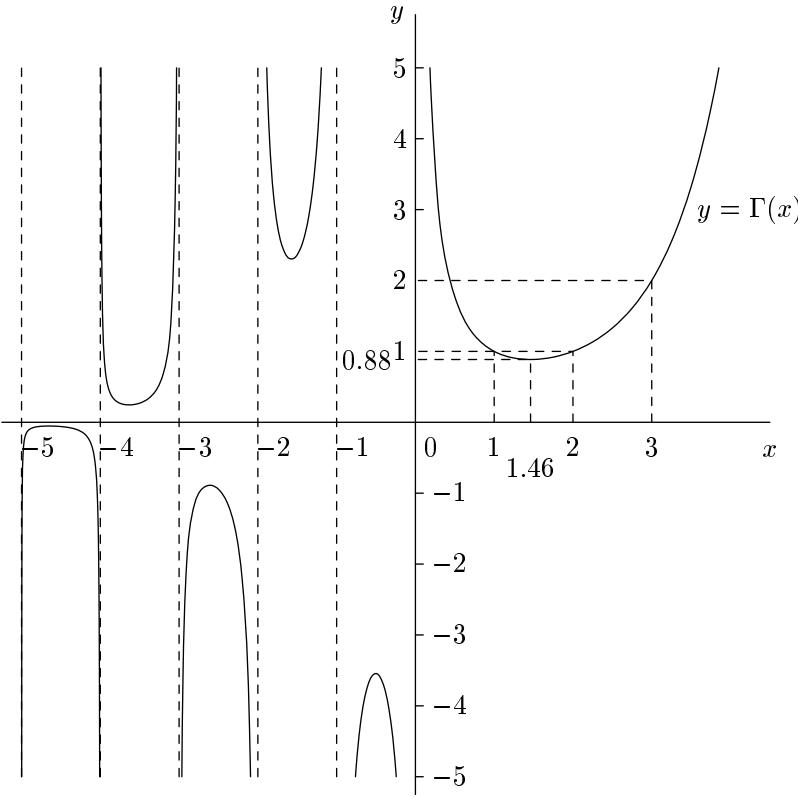
\includegraphics[keepaspectratio]{images/part002_cfbcc1f6.jpg}}\\
图 1\\
因而 \(\Gamma''(x)\) 与 \(\Gamma(x)\) 有相同的符号；于是 \(\Gamma\) 在 x \textgreater{} 0 时以及 \(-(2n + 2) < x < -(2n + 1)\) 时凸，在 \(-(2n + 1) < x - 2n\) 时凹（ \(n \in N\) ）；由此推出，在 \(\Gamma\) 凸的区间上，\(\Gamma'(x)\) 从 \(-\infty\) 递增到 \(+\infty\) ，而在 \(\Gamma\) 凹的区间上，\(\Gamma'(x)\) 从 \(+\infty\) 递减到 \(-\infty\) 。由此得到 \(\Gamma\) 的图像（图 1）。
